% Options for packages loaded elsewhere
\PassOptionsToPackage{unicode}{hyperref}
\PassOptionsToPackage{hyphens}{url}
%
\documentclass[
  letterpaper,
  oneside,
  open=any]{scrbook}

\usepackage{amsmath,amssymb}
\usepackage{iftex}
\ifPDFTeX
  \usepackage[T1]{fontenc}
  \usepackage[utf8]{inputenc}
  \usepackage{textcomp} % provide euro and other symbols
\else % if luatex or xetex
  \usepackage{unicode-math}
  \defaultfontfeatures{Scale=MatchLowercase}
  \defaultfontfeatures[\rmfamily]{Ligatures=TeX,Scale=1}
\fi
\usepackage{lmodern}
\ifPDFTeX\else  
    % xetex/luatex font selection
\fi
% Use upquote if available, for straight quotes in verbatim environments
\IfFileExists{upquote.sty}{\usepackage{upquote}}{}
\IfFileExists{microtype.sty}{% use microtype if available
  \usepackage[]{microtype}
  \UseMicrotypeSet[protrusion]{basicmath} % disable protrusion for tt fonts
}{}
\makeatletter
\@ifundefined{KOMAClassName}{% if non-KOMA class
  \IfFileExists{parskip.sty}{%
    \usepackage{parskip}
  }{% else
    \setlength{\parindent}{0pt}
    \setlength{\parskip}{6pt plus 2pt minus 1pt}}
}{% if KOMA class
  \KOMAoptions{parskip=half}}
\makeatother
\usepackage{xcolor}
\setlength{\emergencystretch}{3em} % prevent overfull lines
\setcounter{secnumdepth}{5}
% Make \paragraph and \subparagraph free-standing
\ifx\paragraph\undefined\else
  \let\oldparagraph\paragraph
  \renewcommand{\paragraph}[1]{\oldparagraph{#1}\mbox{}}
\fi
\ifx\subparagraph\undefined\else
  \let\oldsubparagraph\subparagraph
  \renewcommand{\subparagraph}[1]{\oldsubparagraph{#1}\mbox{}}
\fi

\providecommand{\tightlist}{%
  \setlength{\itemsep}{0pt}\setlength{\parskip}{0pt}}\usepackage{longtable,booktabs,array}
\usepackage{calc} % for calculating minipage widths
% Correct order of tables after \paragraph or \subparagraph
\usepackage{etoolbox}
\makeatletter
\patchcmd\longtable{\par}{\if@noskipsec\mbox{}\fi\par}{}{}
\makeatother
% Allow footnotes in longtable head/foot
\IfFileExists{footnotehyper.sty}{\usepackage{footnotehyper}}{\usepackage{footnote}}
\makesavenoteenv{longtable}
\usepackage{graphicx}
\makeatletter
\def\maxwidth{\ifdim\Gin@nat@width>\linewidth\linewidth\else\Gin@nat@width\fi}
\def\maxheight{\ifdim\Gin@nat@height>\textheight\textheight\else\Gin@nat@height\fi}
\makeatother
% Scale images if necessary, so that they will not overflow the page
% margins by default, and it is still possible to overwrite the defaults
% using explicit options in \includegraphics[width, height, ...]{}
\setkeys{Gin}{width=\maxwidth,height=\maxheight,keepaspectratio}
% Set default figure placement to htbp
\makeatletter
\def\fps@figure{htbp}
\makeatother
% definitions for citeproc citations
\NewDocumentCommand\citeproctext{}{}
\NewDocumentCommand\citeproc{mm}{%
  \begingroup\def\citeproctext{#2}\cite{#1}\endgroup}
\makeatletter
 % allow citations to break across lines
 \let\@cite@ofmt\@firstofone
 % avoid brackets around text for \cite:
 \def\@biblabel#1{}
 \def\@cite#1#2{{#1\if@tempswa , #2\fi}}
\makeatother
\newlength{\cslhangindent}
\setlength{\cslhangindent}{1.5em}
\newlength{\csllabelwidth}
\setlength{\csllabelwidth}{3em}
\newenvironment{CSLReferences}[2] % #1 hanging-indent, #2 entry-spacing
 {\begin{list}{}{%
  \setlength{\itemindent}{0pt}
  \setlength{\leftmargin}{0pt}
  \setlength{\parsep}{0pt}
  % turn on hanging indent if param 1 is 1
  \ifodd #1
   \setlength{\leftmargin}{\cslhangindent}
   \setlength{\itemindent}{-1\cslhangindent}
  \fi
  % set entry spacing
  \setlength{\itemsep}{#2\baselineskip}}}
 {\end{list}}
\usepackage{calc}
\newcommand{\CSLBlock}[1]{\hfill\break\parbox[t]{\linewidth}{\strut\ignorespaces#1\strut}}
\newcommand{\CSLLeftMargin}[1]{\parbox[t]{\csllabelwidth}{\strut#1\strut}}
\newcommand{\CSLRightInline}[1]{\parbox[t]{\linewidth - \csllabelwidth}{\strut#1\strut}}
\newcommand{\CSLIndent}[1]{\hspace{\cslhangindent}#1}

\usepackage{booktabs}
\usepackage{longtable}
\usepackage{array}
\usepackage{multirow}
\usepackage{wrapfig}
\usepackage{float}
\usepackage{colortbl}
\usepackage{pdflscape}
\usepackage{tabu}
\usepackage{threeparttable}
\usepackage{threeparttablex}
\usepackage[normalem]{ulem}
\usepackage{makecell}
\usepackage{xcolor}
\usepackage{fontspec}
\usepackage{multicol}
\usepackage{hhline}
\newlength\Oldarrayrulewidth
\newlength\Oldtabcolsep
\usepackage{hyperref}
\usepackage[default]{opensans}
\fontseries{lc}\selectfont
\makeatletter
\@ifpackageloaded{caption}{}{\usepackage{caption}}
\AtBeginDocument{%
\ifdefined\contentsname
  \renewcommand*\contentsname{Table of contents}
\else
  \newcommand\contentsname{Table of contents}
\fi
\ifdefined\listfigurename
  \renewcommand*\listfigurename{List of Figures}
\else
  \newcommand\listfigurename{List of Figures}
\fi
\ifdefined\listtablename
  \renewcommand*\listtablename{List of Tables}
\else
  \newcommand\listtablename{List of Tables}
\fi
\ifdefined\figurename
  \renewcommand*\figurename{Figure}
\else
  \newcommand\figurename{Figure}
\fi
\ifdefined\tablename
  \renewcommand*\tablename{Table}
\else
  \newcommand\tablename{Table}
\fi
}
\@ifpackageloaded{float}{}{\usepackage{float}}
\floatstyle{ruled}
\@ifundefined{c@chapter}{\newfloat{codelisting}{h}{lop}}{\newfloat{codelisting}{h}{lop}[chapter]}
\floatname{codelisting}{Listing}
\newcommand*\listoflistings{\listof{codelisting}{List of Listings}}
\makeatother
\makeatletter
\makeatother
\makeatletter
\@ifpackageloaded{caption}{}{\usepackage{caption}}
\@ifpackageloaded{subcaption}{}{\usepackage{subcaption}}
\makeatother

\usepackage{hyphenat}
\usepackage{ifthen}
\usepackage{calc}
\usepackage{calculator}

\usepackage{graphicx}
\usepackage{wallpaper}

\usepackage{geometry}

\usepackage{graphicx}
\usepackage{geometry}
\usepackage{afterpage}
\usepackage{tikz}
\usetikzlibrary{calc}
\usetikzlibrary{fadings}
\usepackage[pagecolor=none]{pagecolor}



% Set the titlepage font families







% Set the coverpage font families





\ifLuaTeX
  \usepackage{selnolig}  % disable illegal ligatures
\fi
\usepackage{bookmark}

\IfFileExists{xurl.sty}{\usepackage{xurl}}{} % add URL line breaks if available
\urlstyle{same} % disable monospaced font for URLs
\hypersetup{
  pdftitle={Integrated Ecosystem Assessment Data Guidance Documentation},
  pdfauthor={Integrated Ecosystem Assessment},
  hidelinks,
  pdfcreator={LaTeX via pandoc}}

\title{Integrated Ecosystem Assessment Data Guidance Documentation}
\author{Integrated Ecosystem Assessment}
\date{}

\begin{document}
%%%%% begin titlepage extension code

  \begin{frontmatter}

\begin{titlepage}
% This is a combination of Pandoc templating and LaTeX
% Pandoc templating https://pandoc.org/MANUAL.html#templates
% See the README for help

\thispagestyle{empty}

\newgeometry{top=-100in}

% Page color

\newcommand{\coverauthorstyle}[1]{{\fontsize{20}{24.0}\selectfont
#1}}

\begin{tikzpicture}[remember picture, overlay, inner sep=0pt, outer sep=0pt]

\tikzfading[name=fadeout, inner color=transparent!0,outer color=transparent!100]
\tikzfading[name=fadein, inner color=transparent!100,outer color=transparent!0]
\node[anchor=south west, rotate=0.0, opacity=1.0] at ($(current page.south west)+(0pt, 8.75in)$) {

\includegraphics[width=\paperwidth, keepaspectratio]{img/cover-header-2.png}};

% Title
\newcommand{\titlelocationleft}{2.3in}
\newcommand{\titlelocationbottom}{7in}
\newcommand{\titlealign}{left}

\begin{scope}
{%
\fontsize{30}{36.0}\selectfont
\node[anchor=north
west, align=left, rotate=0] (Title1) at ($(current page.south west)+(\titlelocationleft,\titlelocationbottom)$)  [text width = 5in]  {\textcolor{black}{\bfseries{\nohyphens{Integrated
Ecosystem Assessment Data Guidance Documentation}}}};
}
\end{scope}

% Author
\newcommand{\authorlocationleft}{2.3in}
\newcommand{\authorlocationbottom}{5in}
\newcommand{\authoralign}{left}

\begin{scope}
{%
\fontsize{20}{24.0}\selectfont
\node[anchor=north
west, align=left, rotate=0] (Author1) at ($(current page.south west)+(\authorlocationleft,\authorlocationbottom)$)  [text width = 5in]  {
\coverauthorstyle{Integrated Ecosystem Assessment\\}};
}
\end{scope}

% Header
\newcommand{\headerlocationleft}{2.3in}
\newcommand{\headerlocationbottom}{9.8in}
\newcommand{\headerlocationalign}{left}

\begin{scope}
{%
\fontsize{16}{19.2}\selectfont
 \node[anchor=north west, align=left, rotate=0] (Header1) at %
($(current page.south west)+(\headerlocationleft,\headerlocationbottom)$)  [text width = 5in]  {\textcolor{white}{\nohyphens{NOAA
Technical Memorandum NMFS-XXX-\#\#}}};
}
\end{scope}

% Footer
\newcommand{\footerlocationleft}{6in}
\newcommand{\footerlocationbottom}{0.1\paperheight}
\newcommand{\footerlocationalign}{left}

\begin{scope}
{%
\fontsize{8}{9.6}\selectfont
 \node[anchor=north west, align=left, rotate=0] (Footer1) at %
($(current page.south west)+(\footerlocationleft,\footerlocationbottom)$)  [text width = 2.5in]  {{\nohyphens{U.S.
DEPARTMENT OF COMMERCE\\
\strut \\
National Oceanic and Atmospheric Administration\\
National Marine Fisheries Service\\
Northwest Fisheries Science Center}}};
}
\end{scope}

\end{tikzpicture}
\clearpage
\restoregeometry
%%% TITLE PAGE START

% Set up alignment commands
%Page
\newcommand{\titlepagepagealign}{
\ifthenelse{\equal{left}{right}}{\raggedleft}{}
\ifthenelse{\equal{left}{center}}{\centering}{}
\ifthenelse{\equal{left}{left}}{\raggedright}{}
}
%% Titles
\newcommand{\titlepagetitlealign}{
\ifthenelse{\equal{left}{right}}{\raggedleft}{}
\ifthenelse{\equal{left}{center}}{\centering}{}
\ifthenelse{\equal{left}{left}}{\raggedright}{}
\ifthenelse{\equal{left}{spread}}{\makebox[\linewidth][s]}{}
}


\newcommand{\titleandsubtitle}{
% Title and subtitle
{\fontsize{30}{36.0}\selectfont
\textcolor{black}{\bfseries{\nohyphens{Integrated Ecosystem Assessment
Data Guidance Documentation}}}\par
}%
}
\newcommand{\titlepagetitleblock}{
\titleandsubtitle
}

\newcommand{\authorstyle}[1]{{\fontsize{20}{24.0}\selectfont
#1}}

\newcommand{\affiliationstyle}[1]{{#1}}

\newcommand{\titlepageauthorblock}{
\authorstyle{%
Integrated Ecosystem
Assessment{\textsuperscript{1}}\textsuperscript{,}{\textsuperscript{,*}}
}}

\newcommand{\titlepageaffiliationblock}{
\hangindent=1em
\hangafter=1
\affiliationstyle{
{1}.~enter, enter


\vspace{1\baselineskip} 
* \textit{Correspondence:}~Integrated Ecosystem Assessment~enter
}
}
\newcommand{\headerstyled}{%
{}
}
\newcommand{\footerstyled}{%
{}
}
\newcommand{\datestyled}{%
{}
}


\newcommand{\titlepageheaderblock}{\headerstyled}

\newcommand{\titlepagefooterblock}{
\footerstyled
}

\newcommand{\titlepagedateblock}{
\datestyled
}

%set up blocks so user can specify order
\newcommand{\titleblock}{{\titlepagetitlealign

{\titlepagetitleblock}
}

\vspace{4\baselineskip}
}

\newcommand{\authorblock}{{\titlepageauthorblock}

\vspace{2\baselineskip}
}

\newcommand{\affiliationblock}{{\titlepageaffiliationblock}

\vspace{2\baselineskip}
}

\newcommand{\logoblock}{}

\newcommand{\footerblock}{}

\newcommand{\dateblock}{}

\newcommand{\headerblock}{}
\newgeometry{top=3in,bottom=1in,right=1in,left=1.75in}
% background image
\newlength{\bgimagesize}
\setlength{\bgimagesize}{0.75\paperwidth}
\LENGTHDIVIDE{\bgimagesize}{\paperwidth}{\theRatio} % from calculator pkg
\ThisULCornerWallPaper{\theRatio}{img/corner-image.png}

\thispagestyle{empty} % no page numbers on titlepages


\newcommand{\vrulecode}{\rule{\vrulewidth}{\textheight}}
\newlength{\vrulewidth}
\setlength{\vrulewidth}{0pt}
\newlength{\B}
\setlength{\B}{\ifdim\vrulewidth > 0pt 0.05\textwidth\else 0pt\fi}
\newlength{\minipagewidth}
\ifthenelse{\equal{left}{left} \OR \equal{left}{right} }
{% True case
\setlength{\minipagewidth}{\textwidth - \vrulewidth - \B - 0.1\textwidth}
}{
\setlength{\minipagewidth}{\textwidth - 2\vrulewidth - 2\B - 0.1\textwidth}
}
\ifthenelse{\equal{left}{left} \OR \equal{left}{leftright}}
{% True case
\raggedleft % needed for the minipage to work
\vrulecode
\hspace{\B}
}{%
\raggedright % else it is right only and width is not 0
}
% [position of box][box height][inner position]{width}
% [s] means stretch out vertically; assuming there is a vfill
\begin{minipage}[b][\textheight][s]{\minipagewidth}
\titlepagepagealign
\headerblock

\titleblock

\authorblock

\affiliationblock

\vfill

\logoblock

\footerblock
\par

\end{minipage}\ifthenelse{\equal{left}{right} \OR \equal{left}{leftright} }{
\hspace{\B}
\vrulecode}{}
\clearpage
\restoregeometry
%%% TITLE PAGE END
\end{titlepage}
\setcounter{page}{1}
\end{frontmatter}

%%%%% end titlepage extension code
\renewcommand*\contentsname{Table of contents}
{
\setcounter{tocdepth}{1}
\tableofcontents
}
\listoffigures
\listoftables
\mainmatter
\part{Welcome}

\begin{quote}
Report run date: Wednesday, April 02, 2025
\end{quote}

\section*{Integrated Ecosystem
Assesments}\label{integrated-ecosystem-assesments}
\addcontentsline{toc}{section}{Integrated Ecosystem Assesments}

\markright{Integrated Ecosystem Assesments}

{[}description{]}

\begin{figure}[H]

{\centering 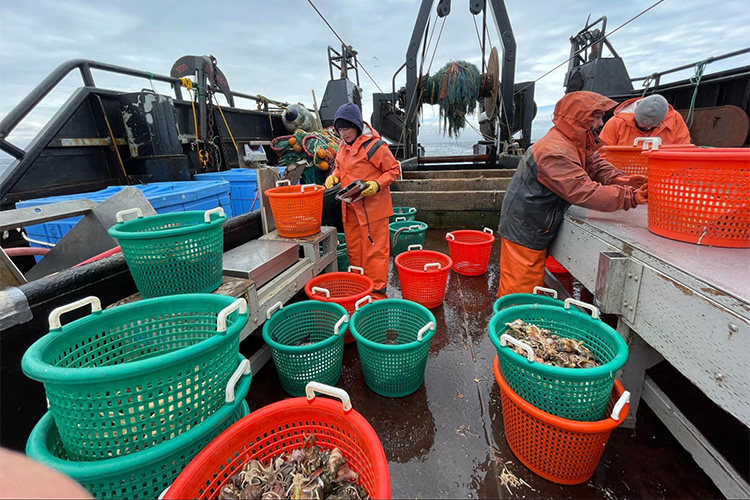
\includegraphics{index_files/mediabag/750x500-bottom-trawl.jpg}

}

\caption{Sorting and weighing fish on deck on the 2022 Bering Sea
groundfish survey aboard the F/V Alaska Knight. Credit: Emily
Markowitz/NOAA Fisheries.}

\end{figure}%

\section*{Documentation Objective}\label{documentation-objective}
\addcontentsline{toc}{section}{Documentation Objective}

\markright{Documentation Objective}

As part of our commitment to open science, reproducibility, and
transparency, we provide this metadata guide to compliment our
public-domain data.

\begin{quote}
Please consider this resource to be a \textbf{Living Document}. The code
in this repository is regularly being updated and improved. Please refer
to
\href{https://github.com/IEA-Data/IEA_Data_Guidance_Doc//releases}{releases}
for finalized products and project milestones.
\end{quote}

\begin{quote}
Do not hesitate to reach out (to us at either {[}email{]} or
\href{https://github.com/IEA-Data/IEA_Data_Guidance_Doc//issues}{GitHub
issues}, especially if you find discrepancies in the data or want to
suggest improvements to infrastructure. Thank you in advance for your
collaboration and partnership with us as we develop our future data
universe.
\end{quote}

\section*{User Resources}\label{user-resources}
\addcontentsline{toc}{section}{User Resources}

\markright{User Resources}

\begin{itemize}
\tightlist
\item
  \href{https://www.integratedecosystemassessment.noaa.gov/ecosystem-status-reports}{IEA
  Ecosystem Status Reports}
\end{itemize}

\section*{Cite this data}\label{cite-this-data}
\addcontentsline{toc}{section}{Cite this data}

\markright{Cite this data}

Use the below
\href{https://github.com/IEA-Data/IEA_Data_Guidance_Doc//blob/main/CITATION.bib}{bibtext
citations}, as cited in our group's
\href{https://github.com/IEA-Data/citations/blob/main/cite/bibliography.bib}{citation
repository} for citing the data created and maintained in this repo. Add
``note = \{Accessed: mm/dd/yyyy\}'' to append the day this data was
accessed. Included here are AFSC RACE Groundfish and Shellfish
Assessment Program's:

\begin{verbatim}

@misc{IEA-Data,
  author = {{National Integrated Ecosystem Assessment Program}},
  title = {National Integrated Ecosystem Assessment Program},
  howpublished = {https://www.integratedecosystemassessment.noaa.gov/ecosystem-status-reports},
  publisher = {{U.S. Dep. Commer.}},
  copyright = {Public Domain} 
}
\end{verbatim}

\section*{Access Constraints}\label{access-constraints}
\addcontentsline{toc}{section}{Access Constraints}

\markright{Access Constraints}

There are no legal restrictions on access to the data. They reside in
public domain and can be freely distributed.

\textbf{User Constraints:} Users must read and fully comprehend the
metadata and
\href{https://IEA-Data.io/IEA_Data_Guidance_Doc/content/code-of-conduct.html}{code
of conduct} prior to use. Data should not be used beyond the limits of
the source scale. Acknowledgement of the Program, as the source from
which these data were obtained, in any publications and/or other
representations of these data, is suggested.

\section*{Suggestions and comments}\label{suggestions-and-comments}
\addcontentsline{toc}{section}{Suggestions and comments}

\markright{Suggestions and comments}

If the data or metadata can be improved, please create a pull request or
\href{https://github.com/IEA-Data/IEA_Data_Guidance_Doc//issues}{submit
an issue to the code's repository}.

\section*{NOAA README}\label{noaa-readme}
\addcontentsline{toc}{section}{NOAA README}

\markright{NOAA README}

This repository is a scientific product and is not official
communication of the National Oceanic and Atmospheric Administration, or
the United States Department of Commerce. All NOAA GitHub project code
is provided on an `as is' basis and the user assumes responsibility for
its use. Any claims against the Department of Commerce or Department of
Commerce bureaus stemming from the use of this GitHub project will be
governed by all applicable Federal law. Any reference to specific
commercial products, processes, or services by service mark, trademark,
manufacturer, or otherwise, does not constitute or imply their
endorsement, recommendation or favoring by the Department of Commerce.
The Department of Commerce seal and logo, or the seal and logo of a DOC
bureau, shall not be used in any manner to imply endorsement of any
commercial product or activity by DOC or the United States Government.

\section*{NOAA License}\label{noaa-license}
\addcontentsline{toc}{section}{NOAA License}

\markright{NOAA License}

Software code created by U.S. Government employees is not subject to
copyright in the United States (17 U.S.C. §105). The United
States/Department of Commerce reserve all rights to seek and obtain
copyright protection in countries other than the United States for
Software authored in its entirety by the Department of Commerce. To this
end, the Department of Commerce hereby grants to Recipient a
royalty-free, nonexclusive license to use, copy, and create derivative
works of the Software outside of the United States.

\chapter{Workflow}\label{workflow}

\section{Operational Product Development
Timeline}\label{operational-product-development-timeline}

Over the course of the year, the survey team is developing a variety of
different data products. Planning and preparation for surveys happens in
the late winter and spring, surveys occur in the summer, data validation
takes place over the course of the survey and after the survey, and data
products are produced through fall and late winter.

\global\setlength{\Oldarrayrulewidth}{\arrayrulewidth}

\global\setlength{\Oldtabcolsep}{\tabcolsep}

\setlength{\tabcolsep}{2pt}

\renewcommand*{\arraystretch}{1.5}



\providecommand{\ascline}[3]{\noalign{\global\arrayrulewidth #1}\arrayrulecolor[HTML]{#2}\cline{#3}}

\begin{longtable}[c]{|p{0.75in}|p{0.75in}|p{0.75in}|p{0.75in}|p{0.75in}|p{0.75in}|p{0.75in}|p{0.75in}|p{0.75in}|p{0.75in}|p{0.75in}|p{0.75in}|p{0.75in}}
\caption{Operational product development timeline.}\tabularnewline




\hhline{>{\arrayrulecolor[HTML]{666666}\global\arrayrulewidth=1.5pt}->{\arrayrulecolor[HTML]{666666}\global\arrayrulewidth=1.5pt}->{\arrayrulecolor[HTML]{666666}\global\arrayrulewidth=1.5pt}->{\arrayrulecolor[HTML]{666666}\global\arrayrulewidth=1.5pt}->{\arrayrulecolor[HTML]{666666}\global\arrayrulewidth=1.5pt}->{\arrayrulecolor[HTML]{666666}\global\arrayrulewidth=1.5pt}->{\arrayrulecolor[HTML]{666666}\global\arrayrulewidth=1.5pt}->{\arrayrulecolor[HTML]{666666}\global\arrayrulewidth=1.5pt}->{\arrayrulecolor[HTML]{666666}\global\arrayrulewidth=1.5pt}->{\arrayrulecolor[HTML]{666666}\global\arrayrulewidth=1.5pt}->{\arrayrulecolor[HTML]{666666}\global\arrayrulewidth=1.5pt}->{\arrayrulecolor[HTML]{666666}\global\arrayrulewidth=1.5pt}->{\arrayrulecolor[HTML]{666666}\global\arrayrulewidth=1.5pt}-}

\multicolumn{1}{>{\raggedright}m{\dimexpr 0.75in+0\tabcolsep}}{\textcolor[HTML]{000000}{\fontsize{11}{11}\selectfont{\global\setmainfont{Arial}{\ }}}} & \multicolumn{1}{!{\color[HTML]{666666}\vrule width 1pt}>{\raggedright}m{\dimexpr 0.75in+0\tabcolsep}}{\textcolor[HTML]{000000}{\fontsize{11}{11}\selectfont{\global\setmainfont{Arial}{January}}}} & \multicolumn{1}{>{\raggedright}m{\dimexpr 0.75in+0\tabcolsep}}{\textcolor[HTML]{000000}{\fontsize{11}{11}\selectfont{\global\setmainfont{Arial}{February}}}} & \multicolumn{1}{>{\raggedright}m{\dimexpr 0.75in+0\tabcolsep}}{\textcolor[HTML]{000000}{\fontsize{11}{11}\selectfont{\global\setmainfont{Arial}{March}}}} & \multicolumn{1}{>{\raggedright}m{\dimexpr 0.75in+0\tabcolsep}}{\textcolor[HTML]{000000}{\fontsize{11}{11}\selectfont{\global\setmainfont{Arial}{April}}}} & \multicolumn{1}{>{\raggedright}m{\dimexpr 0.75in+0\tabcolsep}}{\textcolor[HTML]{000000}{\fontsize{11}{11}\selectfont{\global\setmainfont{Arial}{May}}}} & \multicolumn{1}{>{\raggedright}m{\dimexpr 0.75in+0\tabcolsep}}{\textcolor[HTML]{000000}{\fontsize{11}{11}\selectfont{\global\setmainfont{Arial}{June}}}} & \multicolumn{1}{>{\raggedright}m{\dimexpr 0.75in+0\tabcolsep}}{\textcolor[HTML]{000000}{\fontsize{11}{11}\selectfont{\global\setmainfont{Arial}{July}}}} & \multicolumn{1}{>{\raggedright}m{\dimexpr 0.75in+0\tabcolsep}}{\textcolor[HTML]{000000}{\fontsize{11}{11}\selectfont{\global\setmainfont{Arial}{August}}}} & \multicolumn{1}{>{\raggedright}m{\dimexpr 0.75in+0\tabcolsep}}{\textcolor[HTML]{000000}{\fontsize{11}{11}\selectfont{\global\setmainfont{Arial}{September}}}} & \multicolumn{1}{>{\raggedright}m{\dimexpr 0.75in+0\tabcolsep}}{\textcolor[HTML]{000000}{\fontsize{11}{11}\selectfont{\global\setmainfont{Arial}{October}}}} & \multicolumn{1}{>{\raggedright}m{\dimexpr 0.75in+0\tabcolsep}}{\textcolor[HTML]{000000}{\fontsize{11}{11}\selectfont{\global\setmainfont{Arial}{November}}}} & \multicolumn{1}{>{\raggedright}m{\dimexpr 0.75in+0\tabcolsep}}{\textcolor[HTML]{000000}{\fontsize{11}{11}\selectfont{\global\setmainfont{Arial}{December}}}} \\

\noalign{\global\arrayrulewidth 0pt}\arrayrulecolor[HTML]{000000}

\hhline{>{\arrayrulecolor[HTML]{666666}\global\arrayrulewidth=1.5pt}-|>{\arrayrulecolor[HTML]{666666}\global\arrayrulewidth=1.5pt}->{\arrayrulecolor[HTML]{666666}\global\arrayrulewidth=1.5pt}->{\arrayrulecolor[HTML]{666666}\global\arrayrulewidth=1.5pt}->{\arrayrulecolor[HTML]{666666}\global\arrayrulewidth=1.5pt}->{\arrayrulecolor[HTML]{666666}\global\arrayrulewidth=1.5pt}->{\arrayrulecolor[HTML]{666666}\global\arrayrulewidth=1.5pt}->{\arrayrulecolor[HTML]{666666}\global\arrayrulewidth=1.5pt}->{\arrayrulecolor[HTML]{666666}\global\arrayrulewidth=1.5pt}->{\arrayrulecolor[HTML]{666666}\global\arrayrulewidth=1.5pt}->{\arrayrulecolor[HTML]{666666}\global\arrayrulewidth=1.5pt}->{\arrayrulecolor[HTML]{666666}\global\arrayrulewidth=1.5pt}->{\arrayrulecolor[HTML]{666666}\global\arrayrulewidth=1.5pt}-}\endfirsthead 

\hhline{>{\arrayrulecolor[HTML]{666666}\global\arrayrulewidth=1.5pt}->{\arrayrulecolor[HTML]{666666}\global\arrayrulewidth=1.5pt}->{\arrayrulecolor[HTML]{666666}\global\arrayrulewidth=1.5pt}->{\arrayrulecolor[HTML]{666666}\global\arrayrulewidth=1.5pt}->{\arrayrulecolor[HTML]{666666}\global\arrayrulewidth=1.5pt}->{\arrayrulecolor[HTML]{666666}\global\arrayrulewidth=1.5pt}->{\arrayrulecolor[HTML]{666666}\global\arrayrulewidth=1.5pt}->{\arrayrulecolor[HTML]{666666}\global\arrayrulewidth=1.5pt}->{\arrayrulecolor[HTML]{666666}\global\arrayrulewidth=1.5pt}->{\arrayrulecolor[HTML]{666666}\global\arrayrulewidth=1.5pt}->{\arrayrulecolor[HTML]{666666}\global\arrayrulewidth=1.5pt}->{\arrayrulecolor[HTML]{666666}\global\arrayrulewidth=1.5pt}->{\arrayrulecolor[HTML]{666666}\global\arrayrulewidth=1.5pt}-}

\multicolumn{1}{>{\raggedright}m{\dimexpr 0.75in+0\tabcolsep}}{\textcolor[HTML]{000000}{\fontsize{11}{11}\selectfont{\global\setmainfont{Arial}{\ }}}} & \multicolumn{1}{!{\color[HTML]{666666}\vrule width 1pt}>{\raggedright}m{\dimexpr 0.75in+0\tabcolsep}}{\textcolor[HTML]{000000}{\fontsize{11}{11}\selectfont{\global\setmainfont{Arial}{January}}}} & \multicolumn{1}{>{\raggedright}m{\dimexpr 0.75in+0\tabcolsep}}{\textcolor[HTML]{000000}{\fontsize{11}{11}\selectfont{\global\setmainfont{Arial}{February}}}} & \multicolumn{1}{>{\raggedright}m{\dimexpr 0.75in+0\tabcolsep}}{\textcolor[HTML]{000000}{\fontsize{11}{11}\selectfont{\global\setmainfont{Arial}{March}}}} & \multicolumn{1}{>{\raggedright}m{\dimexpr 0.75in+0\tabcolsep}}{\textcolor[HTML]{000000}{\fontsize{11}{11}\selectfont{\global\setmainfont{Arial}{April}}}} & \multicolumn{1}{>{\raggedright}m{\dimexpr 0.75in+0\tabcolsep}}{\textcolor[HTML]{000000}{\fontsize{11}{11}\selectfont{\global\setmainfont{Arial}{May}}}} & \multicolumn{1}{>{\raggedright}m{\dimexpr 0.75in+0\tabcolsep}}{\textcolor[HTML]{000000}{\fontsize{11}{11}\selectfont{\global\setmainfont{Arial}{June}}}} & \multicolumn{1}{>{\raggedright}m{\dimexpr 0.75in+0\tabcolsep}}{\textcolor[HTML]{000000}{\fontsize{11}{11}\selectfont{\global\setmainfont{Arial}{July}}}} & \multicolumn{1}{>{\raggedright}m{\dimexpr 0.75in+0\tabcolsep}}{\textcolor[HTML]{000000}{\fontsize{11}{11}\selectfont{\global\setmainfont{Arial}{August}}}} & \multicolumn{1}{>{\raggedright}m{\dimexpr 0.75in+0\tabcolsep}}{\textcolor[HTML]{000000}{\fontsize{11}{11}\selectfont{\global\setmainfont{Arial}{September}}}} & \multicolumn{1}{>{\raggedright}m{\dimexpr 0.75in+0\tabcolsep}}{\textcolor[HTML]{000000}{\fontsize{11}{11}\selectfont{\global\setmainfont{Arial}{October}}}} & \multicolumn{1}{>{\raggedright}m{\dimexpr 0.75in+0\tabcolsep}}{\textcolor[HTML]{000000}{\fontsize{11}{11}\selectfont{\global\setmainfont{Arial}{November}}}} & \multicolumn{1}{>{\raggedright}m{\dimexpr 0.75in+0\tabcolsep}}{\textcolor[HTML]{000000}{\fontsize{11}{11}\selectfont{\global\setmainfont{Arial}{December}}}} \\

\noalign{\global\arrayrulewidth 0pt}\arrayrulecolor[HTML]{000000}

\hhline{>{\arrayrulecolor[HTML]{666666}\global\arrayrulewidth=1.5pt}-|>{\arrayrulecolor[HTML]{666666}\global\arrayrulewidth=1.5pt}->{\arrayrulecolor[HTML]{666666}\global\arrayrulewidth=1.5pt}->{\arrayrulecolor[HTML]{666666}\global\arrayrulewidth=1.5pt}->{\arrayrulecolor[HTML]{666666}\global\arrayrulewidth=1.5pt}->{\arrayrulecolor[HTML]{666666}\global\arrayrulewidth=1.5pt}->{\arrayrulecolor[HTML]{666666}\global\arrayrulewidth=1.5pt}->{\arrayrulecolor[HTML]{666666}\global\arrayrulewidth=1.5pt}->{\arrayrulecolor[HTML]{666666}\global\arrayrulewidth=1.5pt}->{\arrayrulecolor[HTML]{666666}\global\arrayrulewidth=1.5pt}->{\arrayrulecolor[HTML]{666666}\global\arrayrulewidth=1.5pt}->{\arrayrulecolor[HTML]{666666}\global\arrayrulewidth=1.5pt}->{\arrayrulecolor[HTML]{666666}\global\arrayrulewidth=1.5pt}-}\endhead



\multicolumn{1}{>{\raggedright}m{\dimexpr 0.75in+0\tabcolsep}}{\textcolor[HTML]{000000}{\fontsize{11}{11}\selectfont{\global\setmainfont{Arial}{Surveys}}}} & \multicolumn{1}{!{\color[HTML]{666666}\vrule width 1pt}>{\raggedright}m{\dimexpr 0.75in+0\tabcolsep}}{\textcolor[HTML]{000000}{\fontsize{11}{11}\selectfont{\global\setmainfont{Arial}{}}}} & \multicolumn{1}{>{\raggedright}m{\dimexpr 0.75in+0\tabcolsep}}{\textcolor[HTML]{000000}{\fontsize{11}{11}\selectfont{\global\setmainfont{Arial}{}}}} & \multicolumn{1}{>{\raggedright}m{\dimexpr 0.75in+0\tabcolsep}}{\textcolor[HTML]{000000}{\fontsize{11}{11}\selectfont{\global\setmainfont{Arial}{}}}} & \multicolumn{1}{>{\raggedright}m{\dimexpr 0.75in+0\tabcolsep}}{\textcolor[HTML]{000000}{\fontsize{11}{11}\selectfont{\global\setmainfont{Arial}{}}}} & \multicolumn{1}{>{\cellcolor[HTML]{382A54}\raggedright}m{\dimexpr 0.75in+0\tabcolsep}}{\textcolor[HTML]{382A54}{\fontsize{11}{11}\selectfont{\global\setmainfont{Arial}{1}}}} & \multicolumn{1}{>{\cellcolor[HTML]{382A54}\raggedright}m{\dimexpr 0.75in+0\tabcolsep}}{\textcolor[HTML]{382A54}{\fontsize{11}{11}\selectfont{\global\setmainfont{Arial}{1}}}} & \multicolumn{1}{>{\cellcolor[HTML]{382A54}\raggedright}m{\dimexpr 0.75in+0\tabcolsep}}{\textcolor[HTML]{382A54}{\fontsize{11}{11}\selectfont{\global\setmainfont{Arial}{1}}}} & \multicolumn{1}{>{\cellcolor[HTML]{382A54}\raggedright}m{\dimexpr 0.75in+0\tabcolsep}}{\textcolor[HTML]{382A54}{\fontsize{11}{11}\selectfont{\global\setmainfont{Arial}{1}}}} & \multicolumn{1}{>{\raggedright}m{\dimexpr 0.75in+0\tabcolsep}}{\textcolor[HTML]{000000}{\fontsize{11}{11}\selectfont{\global\setmainfont{Arial}{}}}} & \multicolumn{1}{>{\raggedright}m{\dimexpr 0.75in+0\tabcolsep}}{\textcolor[HTML]{000000}{\fontsize{11}{11}\selectfont{\global\setmainfont{Arial}{}}}} & \multicolumn{1}{>{\raggedright}m{\dimexpr 0.75in+0\tabcolsep}}{\textcolor[HTML]{000000}{\fontsize{11}{11}\selectfont{\global\setmainfont{Arial}{}}}} & \multicolumn{1}{>{\raggedright}m{\dimexpr 0.75in+0\tabcolsep}}{\textcolor[HTML]{000000}{\fontsize{11}{11}\selectfont{\global\setmainfont{Arial}{}}}} \\

\noalign{\global\arrayrulewidth 0pt}\arrayrulecolor[HTML]{000000}





\multicolumn{1}{>{\raggedright}m{\dimexpr 0.75in+0\tabcolsep}}{\textcolor[HTML]{000000}{\fontsize{11}{11}\selectfont{\global\setmainfont{Arial}{Planning}}}} & \multicolumn{1}{!{\color[HTML]{666666}\vrule width 1pt}>{\cellcolor[HTML]{414081}\raggedright}m{\dimexpr 0.75in+0\tabcolsep}}{\textcolor[HTML]{414081}{\fontsize{11}{11}\selectfont{\global\setmainfont{Arial}{1}}}} & \multicolumn{1}{>{\cellcolor[HTML]{414081}\raggedright}m{\dimexpr 0.75in+0\tabcolsep}}{\textcolor[HTML]{414081}{\fontsize{11}{11}\selectfont{\global\setmainfont{Arial}{1}}}} & \multicolumn{1}{>{\cellcolor[HTML]{414081}\raggedright}m{\dimexpr 0.75in+0\tabcolsep}}{\textcolor[HTML]{414081}{\fontsize{11}{11}\selectfont{\global\setmainfont{Arial}{1}}}} & \multicolumn{1}{>{\raggedright}m{\dimexpr 0.75in+0\tabcolsep}}{\textcolor[HTML]{000000}{\fontsize{11}{11}\selectfont{\global\setmainfont{Arial}{}}}} & \multicolumn{1}{>{\raggedright}m{\dimexpr 0.75in+0\tabcolsep}}{\textcolor[HTML]{000000}{\fontsize{11}{11}\selectfont{\global\setmainfont{Arial}{}}}} & \multicolumn{1}{>{\raggedright}m{\dimexpr 0.75in+0\tabcolsep}}{\textcolor[HTML]{000000}{\fontsize{11}{11}\selectfont{\global\setmainfont{Arial}{}}}} & \multicolumn{1}{>{\raggedright}m{\dimexpr 0.75in+0\tabcolsep}}{\textcolor[HTML]{000000}{\fontsize{11}{11}\selectfont{\global\setmainfont{Arial}{}}}} & \multicolumn{1}{>{\raggedright}m{\dimexpr 0.75in+0\tabcolsep}}{\textcolor[HTML]{000000}{\fontsize{11}{11}\selectfont{\global\setmainfont{Arial}{}}}} & \multicolumn{1}{>{\cellcolor[HTML]{414081}\raggedright}m{\dimexpr 0.75in+0\tabcolsep}}{\textcolor[HTML]{414081}{\fontsize{11}{11}\selectfont{\global\setmainfont{Arial}{1}}}} & \multicolumn{1}{>{\cellcolor[HTML]{414081}\raggedright}m{\dimexpr 0.75in+0\tabcolsep}}{\textcolor[HTML]{414081}{\fontsize{11}{11}\selectfont{\global\setmainfont{Arial}{1}}}} & \multicolumn{1}{>{\cellcolor[HTML]{414081}\raggedright}m{\dimexpr 0.75in+0\tabcolsep}}{\textcolor[HTML]{414081}{\fontsize{11}{11}\selectfont{\global\setmainfont{Arial}{1}}}} & \multicolumn{1}{>{\cellcolor[HTML]{414081}\raggedright}m{\dimexpr 0.75in+0\tabcolsep}}{\textcolor[HTML]{414081}{\fontsize{11}{11}\selectfont{\global\setmainfont{Arial}{1}}}} \\

\noalign{\global\arrayrulewidth 0pt}\arrayrulecolor[HTML]{000000}





\multicolumn{1}{>{\raggedright}m{\dimexpr 0.75in+0\tabcolsep}}{\textcolor[HTML]{000000}{\fontsize{11}{11}\selectfont{\global\setmainfont{Arial}{Development}}}} & \multicolumn{1}{!{\color[HTML]{666666}\vrule width 1pt}>{\cellcolor[HTML]{395D9C}\raggedright}m{\dimexpr 0.75in+0\tabcolsep}}{\textcolor[HTML]{395D9C}{\fontsize{11}{11}\selectfont{\global\setmainfont{Arial}{1}}}} & \multicolumn{1}{>{\cellcolor[HTML]{395D9C}\raggedright}m{\dimexpr 0.75in+0\tabcolsep}}{\textcolor[HTML]{395D9C}{\fontsize{11}{11}\selectfont{\global\setmainfont{Arial}{1}}}} & \multicolumn{1}{>{\cellcolor[HTML]{395D9C}\raggedright}m{\dimexpr 0.75in+0\tabcolsep}}{\textcolor[HTML]{395D9C}{\fontsize{11}{11}\selectfont{\global\setmainfont{Arial}{1}}}} & \multicolumn{1}{>{\cellcolor[HTML]{395D9C}\raggedright}m{\dimexpr 0.75in+0\tabcolsep}}{\textcolor[HTML]{395D9C}{\fontsize{11}{11}\selectfont{\global\setmainfont{Arial}{1}}}} & \multicolumn{1}{>{\cellcolor[HTML]{395D9C}\raggedright}m{\dimexpr 0.75in+0\tabcolsep}}{\textcolor[HTML]{395D9C}{\fontsize{11}{11}\selectfont{\global\setmainfont{Arial}{1}}}} & \multicolumn{1}{>{\raggedright}m{\dimexpr 0.75in+0\tabcolsep}}{\textcolor[HTML]{000000}{\fontsize{11}{11}\selectfont{\global\setmainfont{Arial}{}}}} & \multicolumn{1}{>{\raggedright}m{\dimexpr 0.75in+0\tabcolsep}}{\textcolor[HTML]{000000}{\fontsize{11}{11}\selectfont{\global\setmainfont{Arial}{}}}} & \multicolumn{1}{>{\raggedright}m{\dimexpr 0.75in+0\tabcolsep}}{\textcolor[HTML]{000000}{\fontsize{11}{11}\selectfont{\global\setmainfont{Arial}{}}}} & \multicolumn{1}{>{\raggedright}m{\dimexpr 0.75in+0\tabcolsep}}{\textcolor[HTML]{000000}{\fontsize{11}{11}\selectfont{\global\setmainfont{Arial}{}}}} & \multicolumn{1}{>{\cellcolor[HTML]{395D9C}\raggedright}m{\dimexpr 0.75in+0\tabcolsep}}{\textcolor[HTML]{395D9C}{\fontsize{11}{11}\selectfont{\global\setmainfont{Arial}{1}}}} & \multicolumn{1}{>{\cellcolor[HTML]{395D9C}\raggedright}m{\dimexpr 0.75in+0\tabcolsep}}{\textcolor[HTML]{395D9C}{\fontsize{11}{11}\selectfont{\global\setmainfont{Arial}{1}}}} & \multicolumn{1}{>{\cellcolor[HTML]{395D9C}\raggedright}m{\dimexpr 0.75in+0\tabcolsep}}{\textcolor[HTML]{395D9C}{\fontsize{11}{11}\selectfont{\global\setmainfont{Arial}{1}}}} \\

\noalign{\global\arrayrulewidth 0pt}\arrayrulecolor[HTML]{000000}





\multicolumn{1}{>{\raggedright}m{\dimexpr 0.75in+0\tabcolsep}}{\textcolor[HTML]{000000}{\fontsize{11}{11}\selectfont{\global\setmainfont{Arial}{Deployment\ (survey\ deliverables)}}}} & \multicolumn{1}{!{\color[HTML]{666666}\vrule width 1pt}>{\raggedright}m{\dimexpr 0.75in+0\tabcolsep}}{\textcolor[HTML]{000000}{\fontsize{11}{11}\selectfont{\global\setmainfont{Arial}{}}}} & \multicolumn{1}{>{\raggedright}m{\dimexpr 0.75in+0\tabcolsep}}{\textcolor[HTML]{000000}{\fontsize{11}{11}\selectfont{\global\setmainfont{Arial}{}}}} & \multicolumn{1}{>{\raggedright}m{\dimexpr 0.75in+0\tabcolsep}}{\textcolor[HTML]{000000}{\fontsize{11}{11}\selectfont{\global\setmainfont{Arial}{}}}} & \multicolumn{1}{>{\raggedright}m{\dimexpr 0.75in+0\tabcolsep}}{\textcolor[HTML]{000000}{\fontsize{11}{11}\selectfont{\global\setmainfont{Arial}{}}}} & \multicolumn{1}{>{\raggedright}m{\dimexpr 0.75in+0\tabcolsep}}{\textcolor[HTML]{000000}{\fontsize{11}{11}\selectfont{\global\setmainfont{Arial}{}}}} & \multicolumn{1}{>{\raggedright}m{\dimexpr 0.75in+0\tabcolsep}}{\textcolor[HTML]{000000}{\fontsize{11}{11}\selectfont{\global\setmainfont{Arial}{}}}} & \multicolumn{1}{>{\raggedright}m{\dimexpr 0.75in+0\tabcolsep}}{\textcolor[HTML]{000000}{\fontsize{11}{11}\selectfont{\global\setmainfont{Arial}{}}}} & \multicolumn{1}{>{\raggedright}m{\dimexpr 0.75in+0\tabcolsep}}{\textcolor[HTML]{000000}{\fontsize{11}{11}\selectfont{\global\setmainfont{Arial}{}}}} & \multicolumn{1}{>{\cellcolor[HTML]{357BA2}\raggedright}m{\dimexpr 0.75in+0\tabcolsep}}{\textcolor[HTML]{357BA2}{\fontsize{11}{11}\selectfont{\global\setmainfont{Arial}{1}}}} & \multicolumn{1}{>{\cellcolor[HTML]{357BA2}\raggedright}m{\dimexpr 0.75in+0\tabcolsep}}{\textcolor[HTML]{357BA2}{\fontsize{11}{11}\selectfont{\global\setmainfont{Arial}{1}}}} & \multicolumn{1}{>{\cellcolor[HTML]{357BA2}\raggedright}m{\dimexpr 0.75in+0\tabcolsep}}{\textcolor[HTML]{357BA2}{\fontsize{11}{11}\selectfont{\global\setmainfont{Arial}{1}}}} & \multicolumn{1}{>{\cellcolor[HTML]{357BA2}\raggedright}m{\dimexpr 0.75in+0\tabcolsep}}{\textcolor[HTML]{357BA2}{\fontsize{11}{11}\selectfont{\global\setmainfont{Arial}{1}}}} \\

\noalign{\global\arrayrulewidth 0pt}\arrayrulecolor[HTML]{000000}





\multicolumn{1}{>{\raggedright}m{\dimexpr 0.75in+0\tabcolsep}}{\textcolor[HTML]{000000}{\fontsize{11}{11}\selectfont{\global\setmainfont{Arial}{Deployment\ (survey\ operations)}}}} & \multicolumn{1}{!{\color[HTML]{666666}\vrule width 1pt}>{\raggedright}m{\dimexpr 0.75in+0\tabcolsep}}{\textcolor[HTML]{000000}{\fontsize{11}{11}\selectfont{\global\setmainfont{Arial}{}}}} & \multicolumn{1}{>{\raggedright}m{\dimexpr 0.75in+0\tabcolsep}}{\textcolor[HTML]{000000}{\fontsize{11}{11}\selectfont{\global\setmainfont{Arial}{}}}} & \multicolumn{1}{>{\raggedright}m{\dimexpr 0.75in+0\tabcolsep}}{\textcolor[HTML]{000000}{\fontsize{11}{11}\selectfont{\global\setmainfont{Arial}{}}}} & \multicolumn{1}{>{\raggedright}m{\dimexpr 0.75in+0\tabcolsep}}{\textcolor[HTML]{000000}{\fontsize{11}{11}\selectfont{\global\setmainfont{Arial}{}}}} & \multicolumn{1}{>{\cellcolor[HTML]{3497A9}\raggedright}m{\dimexpr 0.75in+0\tabcolsep}}{\textcolor[HTML]{3497A9}{\fontsize{11}{11}\selectfont{\global\setmainfont{Arial}{1}}}} & \multicolumn{1}{>{\cellcolor[HTML]{3497A9}\raggedright}m{\dimexpr 0.75in+0\tabcolsep}}{\textcolor[HTML]{3497A9}{\fontsize{11}{11}\selectfont{\global\setmainfont{Arial}{1}}}} & \multicolumn{1}{>{\cellcolor[HTML]{3497A9}\raggedright}m{\dimexpr 0.75in+0\tabcolsep}}{\textcolor[HTML]{3497A9}{\fontsize{11}{11}\selectfont{\global\setmainfont{Arial}{1}}}} & \multicolumn{1}{>{\cellcolor[HTML]{3497A9}\raggedright}m{\dimexpr 0.75in+0\tabcolsep}}{\textcolor[HTML]{3497A9}{\fontsize{11}{11}\selectfont{\global\setmainfont{Arial}{1}}}} & \multicolumn{1}{>{\raggedright}m{\dimexpr 0.75in+0\tabcolsep}}{\textcolor[HTML]{000000}{\fontsize{11}{11}\selectfont{\global\setmainfont{Arial}{}}}} & \multicolumn{1}{>{\raggedright}m{\dimexpr 0.75in+0\tabcolsep}}{\textcolor[HTML]{000000}{\fontsize{11}{11}\selectfont{\global\setmainfont{Arial}{}}}} & \multicolumn{1}{>{\raggedright}m{\dimexpr 0.75in+0\tabcolsep}}{\textcolor[HTML]{000000}{\fontsize{11}{11}\selectfont{\global\setmainfont{Arial}{}}}} & \multicolumn{1}{>{\raggedright}m{\dimexpr 0.75in+0\tabcolsep}}{\textcolor[HTML]{000000}{\fontsize{11}{11}\selectfont{\global\setmainfont{Arial}{}}}} \\

\noalign{\global\arrayrulewidth 0pt}\arrayrulecolor[HTML]{000000}





\multicolumn{1}{>{\raggedright}m{\dimexpr 0.75in+0\tabcolsep}}{\textcolor[HTML]{000000}{\fontsize{11}{11}\selectfont{\global\setmainfont{Arial}{Triage\ (fixing\ bugs\ and\ errors)}}}} & \multicolumn{1}{!{\color[HTML]{666666}\vrule width 1pt}>{\cellcolor[HTML]{3DB4AD}\raggedright}m{\dimexpr 0.75in+0\tabcolsep}}{\textcolor[HTML]{3DB4AD}{\fontsize{11}{11}\selectfont{\global\setmainfont{Arial}{1}}}} & \multicolumn{1}{>{\cellcolor[HTML]{3DB4AD}\raggedright}m{\dimexpr 0.75in+0\tabcolsep}}{\textcolor[HTML]{3DB4AD}{\fontsize{11}{11}\selectfont{\global\setmainfont{Arial}{1}}}} & \multicolumn{1}{>{\cellcolor[HTML]{3DB4AD}\raggedright}m{\dimexpr 0.75in+0\tabcolsep}}{\textcolor[HTML]{3DB4AD}{\fontsize{11}{11}\selectfont{\global\setmainfont{Arial}{1}}}} & \multicolumn{1}{>{\cellcolor[HTML]{3DB4AD}\raggedright}m{\dimexpr 0.75in+0\tabcolsep}}{\textcolor[HTML]{3DB4AD}{\fontsize{11}{11}\selectfont{\global\setmainfont{Arial}{1}}}} & \multicolumn{1}{>{\cellcolor[HTML]{3DB4AD}\raggedright}m{\dimexpr 0.75in+0\tabcolsep}}{\textcolor[HTML]{3DB4AD}{\fontsize{11}{11}\selectfont{\global\setmainfont{Arial}{1}}}} & \multicolumn{1}{>{\cellcolor[HTML]{3DB4AD}\raggedright}m{\dimexpr 0.75in+0\tabcolsep}}{\textcolor[HTML]{3DB4AD}{\fontsize{11}{11}\selectfont{\global\setmainfont{Arial}{1}}}} & \multicolumn{1}{>{\cellcolor[HTML]{3DB4AD}\raggedright}m{\dimexpr 0.75in+0\tabcolsep}}{\textcolor[HTML]{3DB4AD}{\fontsize{11}{11}\selectfont{\global\setmainfont{Arial}{1}}}} & \multicolumn{1}{>{\cellcolor[HTML]{3DB4AD}\raggedright}m{\dimexpr 0.75in+0\tabcolsep}}{\textcolor[HTML]{3DB4AD}{\fontsize{11}{11}\selectfont{\global\setmainfont{Arial}{1}}}} & \multicolumn{1}{>{\cellcolor[HTML]{3DB4AD}\raggedright}m{\dimexpr 0.75in+0\tabcolsep}}{\textcolor[HTML]{3DB4AD}{\fontsize{11}{11}\selectfont{\global\setmainfont{Arial}{1}}}} & \multicolumn{1}{>{\cellcolor[HTML]{3DB4AD}\raggedright}m{\dimexpr 0.75in+0\tabcolsep}}{\textcolor[HTML]{3DB4AD}{\fontsize{11}{11}\selectfont{\global\setmainfont{Arial}{1}}}} & \multicolumn{1}{>{\cellcolor[HTML]{3DB4AD}\raggedright}m{\dimexpr 0.75in+0\tabcolsep}}{\textcolor[HTML]{3DB4AD}{\fontsize{11}{11}\selectfont{\global\setmainfont{Arial}{1}}}} & \multicolumn{1}{>{\cellcolor[HTML]{3DB4AD}\raggedright}m{\dimexpr 0.75in+0\tabcolsep}}{\textcolor[HTML]{3DB4AD}{\fontsize{11}{11}\selectfont{\global\setmainfont{Arial}{1}}}} \\

\noalign{\global\arrayrulewidth 0pt}\arrayrulecolor[HTML]{000000}





\multicolumn{1}{>{\raggedright}m{\dimexpr 0.75in+0\tabcolsep}}{\textcolor[HTML]{000000}{\fontsize{11}{11}\selectfont{\global\setmainfont{Arial}{User\ feedback\ and\ brainstorming}}}} & \multicolumn{1}{!{\color[HTML]{666666}\vrule width 1pt}>{\cellcolor[HTML]{60CEAC}\raggedright}m{\dimexpr 0.75in+0\tabcolsep}}{\textcolor[HTML]{60CEAC}{\fontsize{11}{11}\selectfont{\global\setmainfont{Arial}{1}}}} & \multicolumn{1}{>{\cellcolor[HTML]{60CEAC}\raggedright}m{\dimexpr 0.75in+0\tabcolsep}}{\textcolor[HTML]{60CEAC}{\fontsize{11}{11}\selectfont{\global\setmainfont{Arial}{1}}}} & \multicolumn{1}{>{\cellcolor[HTML]{60CEAC}\raggedright}m{\dimexpr 0.75in+0\tabcolsep}}{\textcolor[HTML]{60CEAC}{\fontsize{11}{11}\selectfont{\global\setmainfont{Arial}{1}}}} & \multicolumn{1}{>{\cellcolor[HTML]{60CEAC}\raggedright}m{\dimexpr 0.75in+0\tabcolsep}}{\textcolor[HTML]{60CEAC}{\fontsize{11}{11}\selectfont{\global\setmainfont{Arial}{1}}}} & \multicolumn{1}{>{\cellcolor[HTML]{60CEAC}\raggedright}m{\dimexpr 0.75in+0\tabcolsep}}{\textcolor[HTML]{60CEAC}{\fontsize{11}{11}\selectfont{\global\setmainfont{Arial}{1}}}} & \multicolumn{1}{>{\cellcolor[HTML]{60CEAC}\raggedright}m{\dimexpr 0.75in+0\tabcolsep}}{\textcolor[HTML]{60CEAC}{\fontsize{11}{11}\selectfont{\global\setmainfont{Arial}{1}}}} & \multicolumn{1}{>{\cellcolor[HTML]{60CEAC}\raggedright}m{\dimexpr 0.75in+0\tabcolsep}}{\textcolor[HTML]{60CEAC}{\fontsize{11}{11}\selectfont{\global\setmainfont{Arial}{1}}}} & \multicolumn{1}{>{\cellcolor[HTML]{60CEAC}\raggedright}m{\dimexpr 0.75in+0\tabcolsep}}{\textcolor[HTML]{60CEAC}{\fontsize{11}{11}\selectfont{\global\setmainfont{Arial}{1}}}} & \multicolumn{1}{>{\cellcolor[HTML]{60CEAC}\raggedright}m{\dimexpr 0.75in+0\tabcolsep}}{\textcolor[HTML]{60CEAC}{\fontsize{11}{11}\selectfont{\global\setmainfont{Arial}{1}}}} & \multicolumn{1}{>{\cellcolor[HTML]{60CEAC}\raggedright}m{\dimexpr 0.75in+0\tabcolsep}}{\textcolor[HTML]{60CEAC}{\fontsize{11}{11}\selectfont{\global\setmainfont{Arial}{1}}}} & \multicolumn{1}{>{\cellcolor[HTML]{60CEAC}\raggedright}m{\dimexpr 0.75in+0\tabcolsep}}{\textcolor[HTML]{60CEAC}{\fontsize{11}{11}\selectfont{\global\setmainfont{Arial}{1}}}} & \multicolumn{1}{>{\cellcolor[HTML]{60CEAC}\raggedright}m{\dimexpr 0.75in+0\tabcolsep}}{\textcolor[HTML]{60CEAC}{\fontsize{11}{11}\selectfont{\global\setmainfont{Arial}{1}}}} \\

\noalign{\global\arrayrulewidth 0pt}\arrayrulecolor[HTML]{000000}

\hhline{>{\arrayrulecolor[HTML]{666666}\global\arrayrulewidth=1.5pt}-|>{\arrayrulecolor[HTML]{666666}\global\arrayrulewidth=1.5pt}->{\arrayrulecolor[HTML]{666666}\global\arrayrulewidth=1.5pt}->{\arrayrulecolor[HTML]{666666}\global\arrayrulewidth=1.5pt}->{\arrayrulecolor[HTML]{666666}\global\arrayrulewidth=1.5pt}->{\arrayrulecolor[HTML]{666666}\global\arrayrulewidth=1.5pt}->{\arrayrulecolor[HTML]{666666}\global\arrayrulewidth=1.5pt}->{\arrayrulecolor[HTML]{666666}\global\arrayrulewidth=1.5pt}->{\arrayrulecolor[HTML]{666666}\global\arrayrulewidth=1.5pt}->{\arrayrulecolor[HTML]{666666}\global\arrayrulewidth=1.5pt}->{\arrayrulecolor[HTML]{666666}\global\arrayrulewidth=1.5pt}->{\arrayrulecolor[HTML]{666666}\global\arrayrulewidth=1.5pt}->{\arrayrulecolor[HTML]{666666}\global\arrayrulewidth=1.5pt}-}



\end{longtable}



\arrayrulecolor[HTML]{000000}

\global\setlength{\arrayrulewidth}{\Oldarrayrulewidth}

\global\setlength{\tabcolsep}{\Oldtabcolsep}

\renewcommand*{\arraystretch}{1}

\section{Data workflow from boat to
production}\label{data-workflow-from-boat-to-production}

Organisms first need to be collected aboard the vessel before data can
be entered into tablets.

\begin{figure}

\centering{

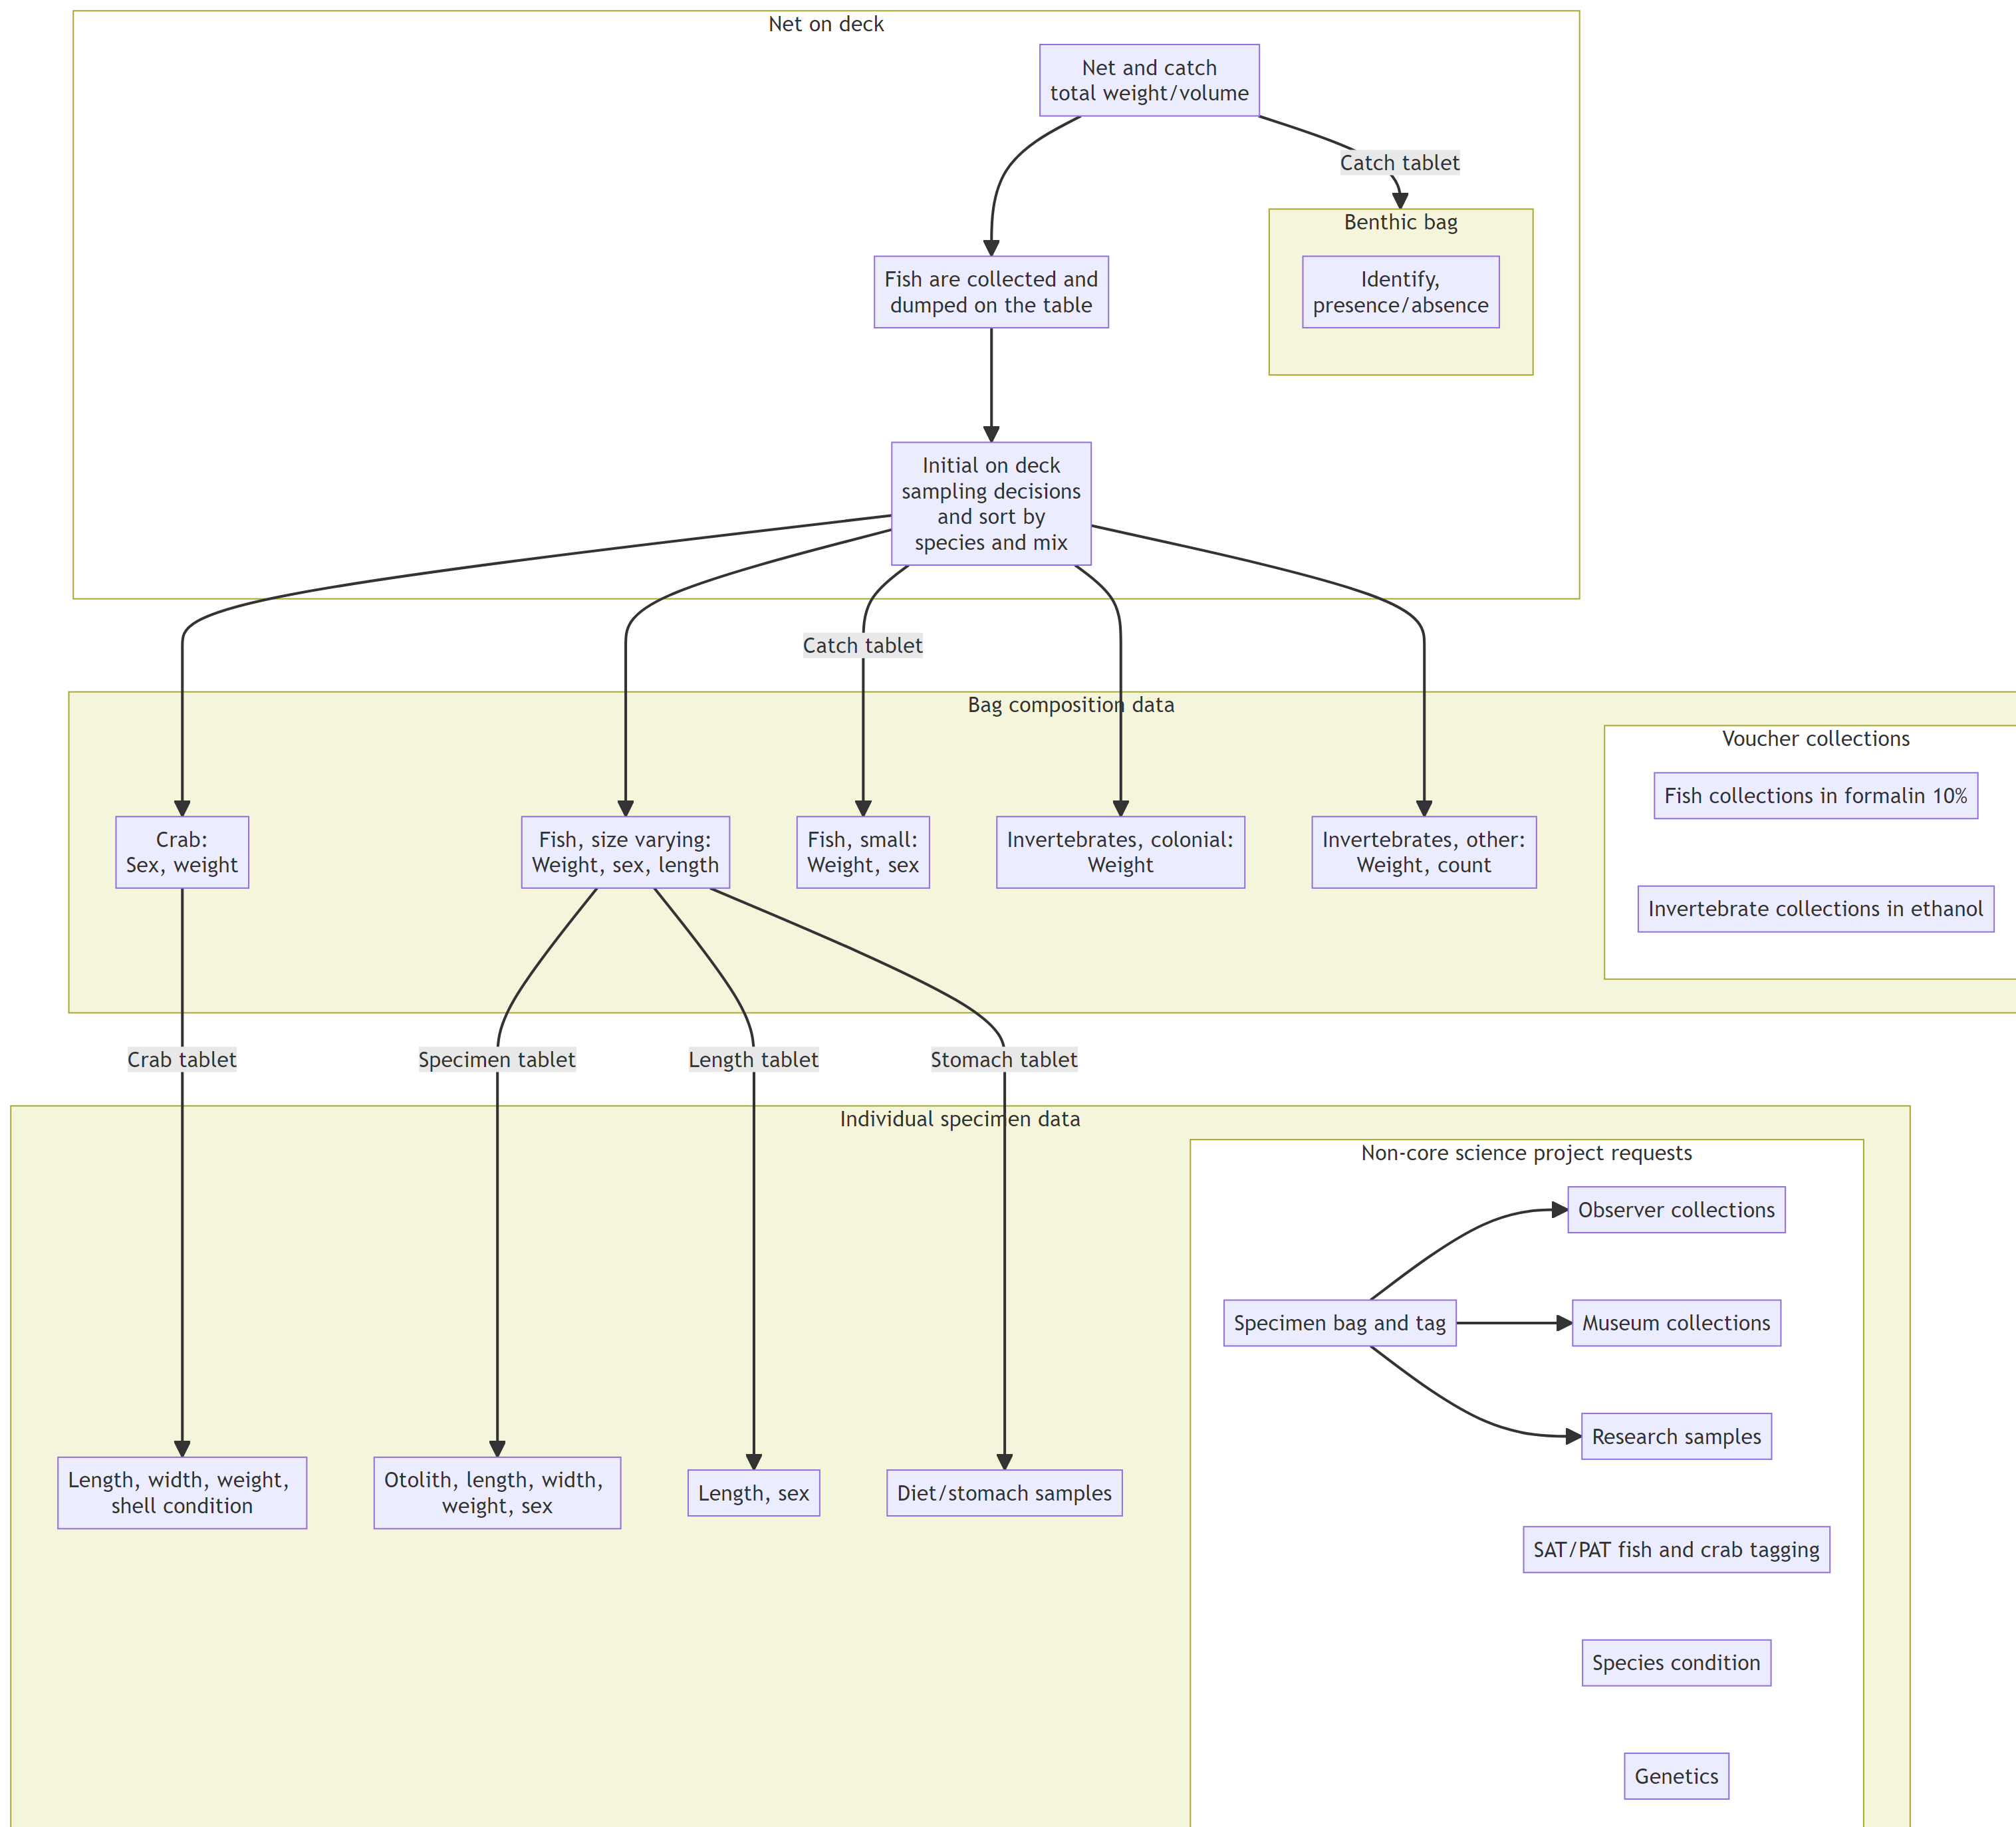
\includegraphics[width=16.11in,height=14.6in]{content/intro-workflow_files/figure-latex/mermaid-figure-1.png}

}

\caption{\label{fig-deck-bio-workflow}Simplified boat deck processing
workflow.}

\end{figure}%

The objective of this process is to take raw data, QA/QC and clean these
data, curate standard data products for these survey. Please note,
through this process we are not providing ``data'' (what we consider
lower level data material; see the data levels section below) but ``data
products'', which is intended to facilitate the most fool-proof standard
interpretation of the data. These data products only use data from
standard and validated hauls, and has undergone careful review.

\textbf{Once survey data collected on the vessel has been checked and
validated}, the
\href{https://github.com/afsc-gap-products/gap_products/blob/main/code/run.R}{\texttt{gap\_products/code/run.R}}
script is used to orchestrate a sequence of programs that calculate the
standard data products resulting from the NOAA AFSC GAP bottom trawl
surveys. Standard data products are the CPUE, BIOMASS, SIZECOMP, and
AGECOMP tables in the \texttt{GAP\_PRODUCTS} Oracle schema. The tables
are slated to be updated twice a year: once after the survey season
following finalization of that summer's bottom trawl survey data to
incorporate the new catch, size, and effort data and once prior to an
upcoming survey to incorporate new age data that were processed after
the prior summer's survey season ended. This second pre-survey
production run will also incorporate changes in the data due to the
specimen voucher process as well as other post-hoc changes in the survey
data.

\begin{quote}
The data from these surveys constitute a \textbf{living data set} so we
can continue to \textbf{provide the best available data to all partners,
stakeholders, and fellow scientists}.
\end{quote}

\begin{figure}

\centering{

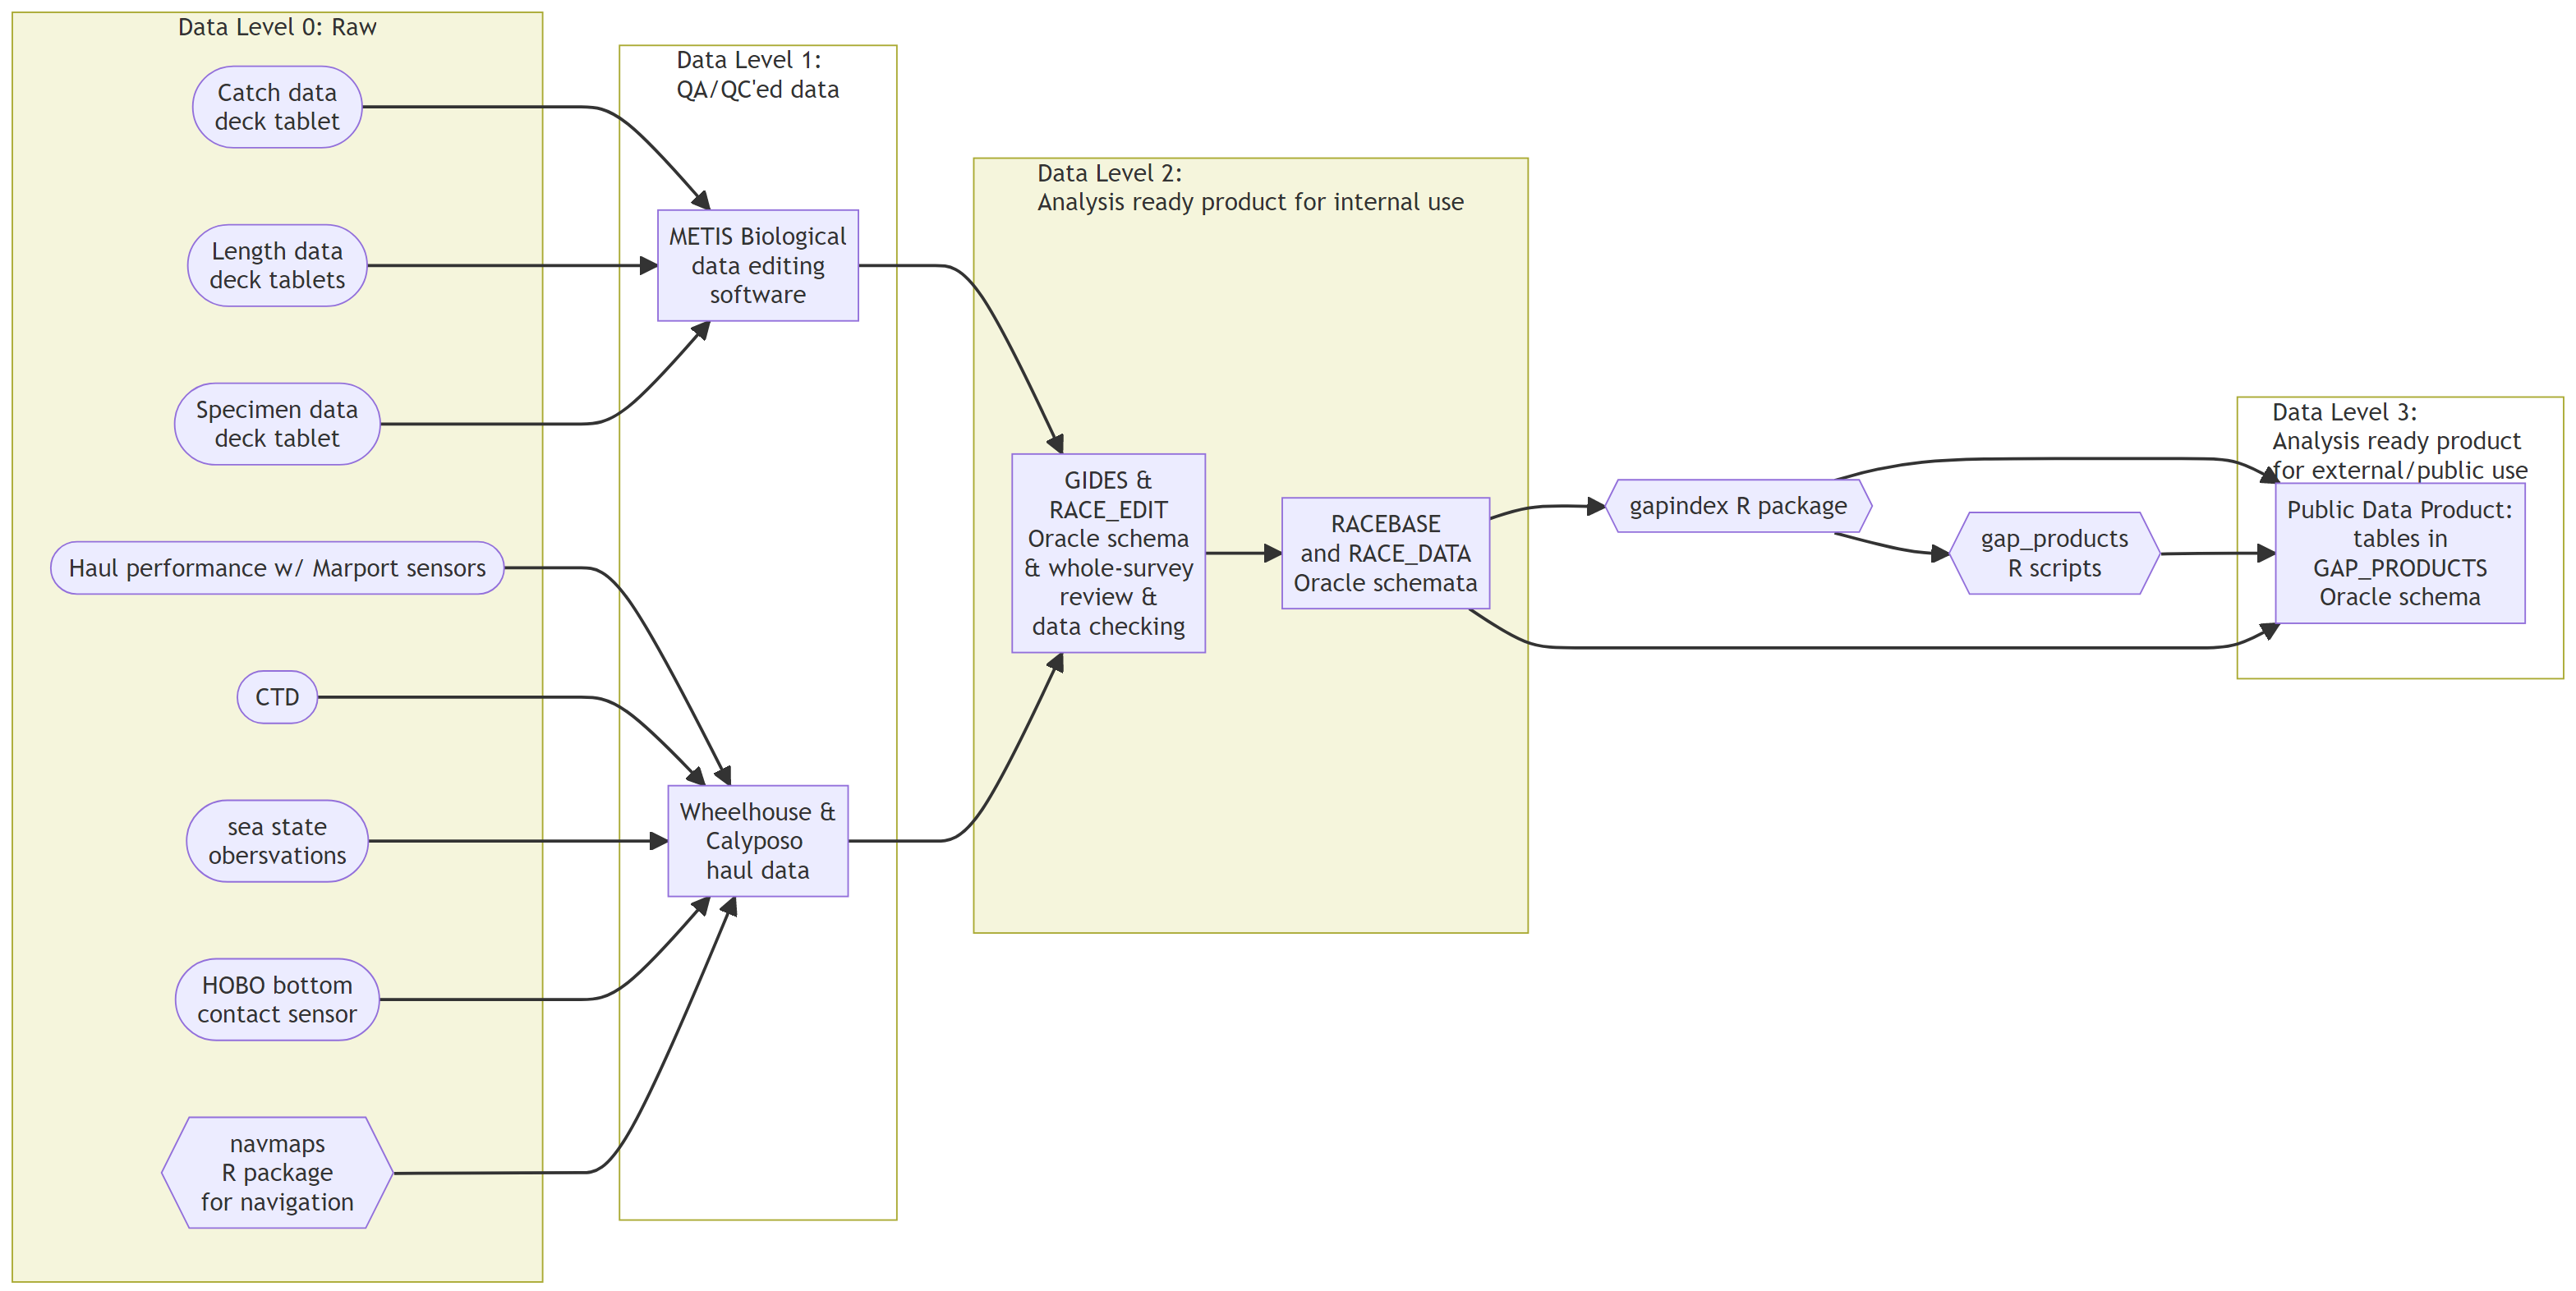
\includegraphics[width=17.45in,height=8.76in]{content/intro-workflow_files/figure-latex/mermaid-figure-3.png}

}

\caption{\label{fig-workflow}Simplified data workflow from boat to
production.}

\end{figure}%

During each data product run cycle:

\begin{enumerate}
\def\labelenumi{\arabic{enumi}.}
\item
  Versions of the tables in GAP\_PRODUCTS are locally imported within
  the gap\_products repository to compare with the updated production
  tables. Any changes to a production table will be compared and checked
  to make sure those changes are intentional and documented.
\item
  Use the \texttt{gapindex} R package to calculate the four major
  standard data products: CPUE, BIOMASS, SIZECOMP, AGECOMP. These tables
  are compared and checked to their respective locally saved copies and
  any changes to the tables are vetted and documented. These tables are
  then uploaded to the GAP\_PRODUCTS Oracle schema.
\item
  Calculate the various materialized views for AKFIN and FOSS purposes.
  Since these are derivative of the tables in GAP\_PRODUCTS as well as
  other base tables in RACEBASE and RACE\_DATA, it is not necessary to
  check these views in addition to the data checks done in the previous
  steps.
\end{enumerate}

\begin{figure}

\centering{

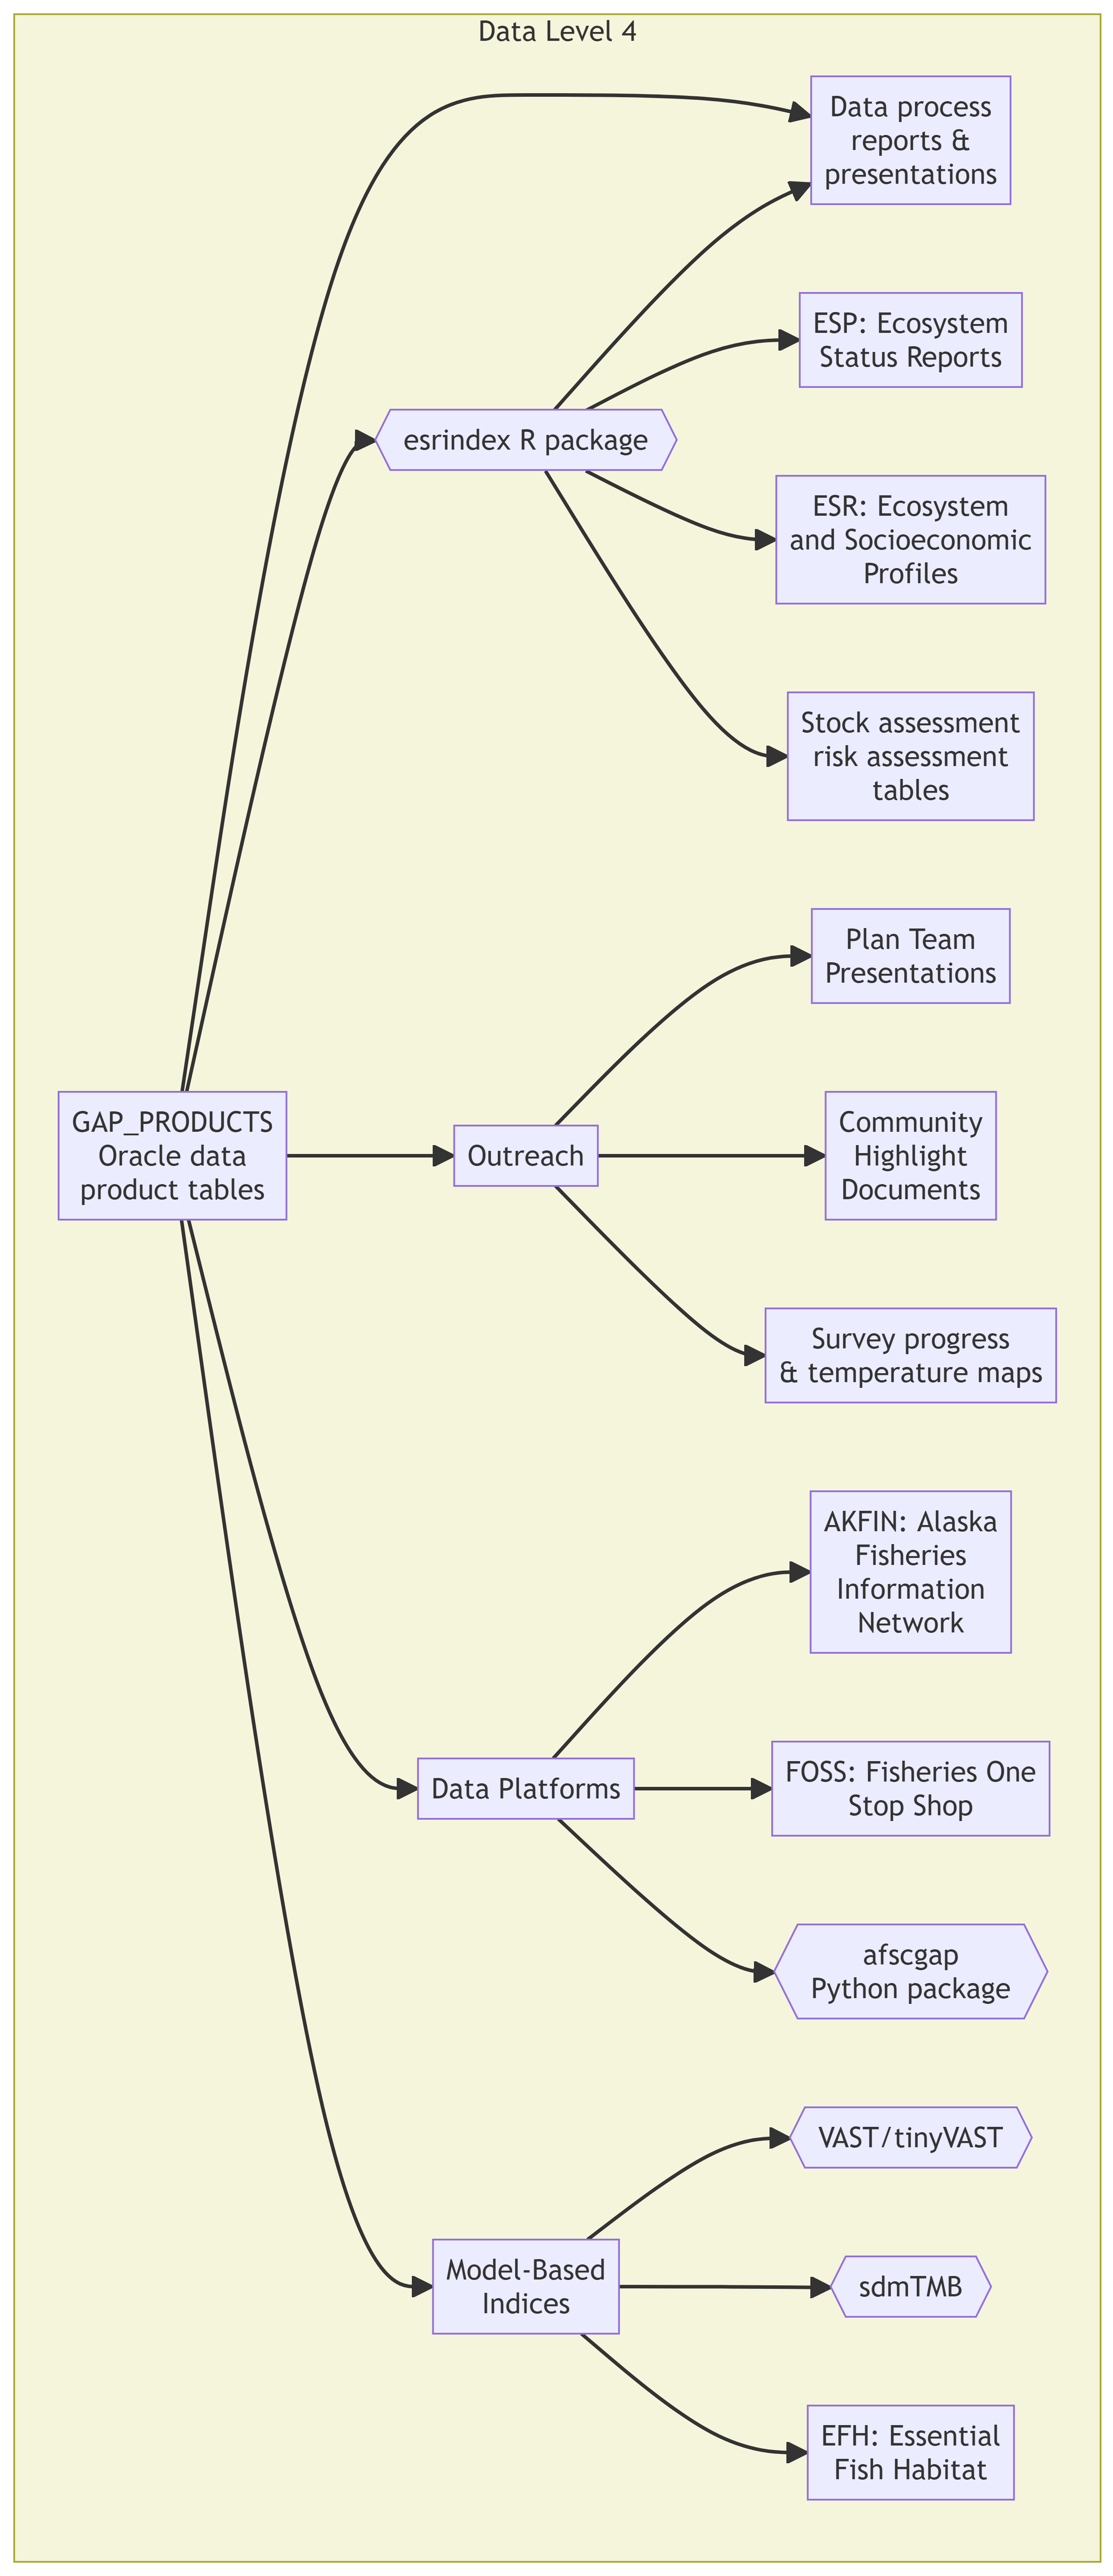
\includegraphics[width=6.54in,height=15.11in]{content/intro-workflow_files/figure-latex/mermaid-figure-2.png}

}

\caption{\label{fig-data-used}Major end-users of the GAP data product
tables.}

\end{figure}%

\section{Data levels}\label{data-levels}

GAP produces numerous data products that are subjected to different
levels of processing, ranging from raw to highly-derived. The
suitability of these data products for analysis varies and there is
ambiguity about which data products can be used for which purpose. This
ambiguity can create challenges in communicating about data products and
potentially lead to misunderstanding and misuse of data. One approach to
communicating about the level of processing applied to data products and
their suitability for analysis is to describe data products using a Data
Processing Level system. Data Processing Level systems are widely used
in earth system sciences to characterize the extent of processing that
has been applied to data products. For example, the NOAA National
Centers for Environmental Information (NCEI) Satellite Program uses a
Data Processing Level system to describe data on a scale of 0-4, where
Level 0 is raw data and Level 4 is model output or results from
analysis. Example of how
\href{https://ladsweb.modaps.eosdis.nasa.gov/search/}{NASA remote
sensing data products} are shared through a public data portal with
levels of data processing and documentation.

For more information, see
\href{https://docs.google.com/presentation/d/1rWSZpeghWJqzWMIa5oBc4BCoy-zy1Yue86RoTw58u6M/edit?usp=sharing}{Sean
Rohan's October 2022 SCRUGS presentation} on the topic.

\begin{itemize}
\tightlist
\item
  \textbf{Level 0}: Raw and unprocessed data. Ex: Data on the G drive,
  some tables in RACE\_DATA
\item
  \textbf{Level 1}: Data products with QA/QC applied that may or may not
  be expanded to analysis units, but either not georeferenced or does
  not include full metadata. Ex: Some tables in RACE\_DATA and RACEBASE
\item
  \textbf{Level 2}: Analysis-ready data products that are derived for a
  standardized extent and account for zeros and missing/bad data. Ex:
  CPUE tables, some data products in public-facing archives and
  repositories
\item
  \textbf{Level 3}: Data products that are synthesized across a
  standardized extent, often inputs in a higher-level analytical
  product. Ex: Abundance indices, some data products in public-facing
  archives and repositories
\item
  \textbf{Level 4}: Analytically generated data products that are
  derived from lower-level data, often to inform management. Ex:
  Biological reference points from stock assessments, Essential Fish
  Habitat layers, indicators in Ecosystem Status Reports and Ecosystem
  and Socioeconomic Profiles
\end{itemize}

\chapter{News}\label{news}

\section{News/change logs}\label{newschange-logs}

--
\href{https://raw.githubusercontent.com/IEA-Data/IEA_Data_Guidance_Doc/main/content/intro-news/2025-04-02.txt}{Run
2025-04-02 Initial Run}: Initial compiling and planning notes

\chapter{Code of Conduct}\label{code-of-conduct}

\section{What are Codes of Conduct?}\label{what-are-codes-of-conduct}

Codes of Conduct are voluntary sets of rules that assist creators,
developers, and users of code and data with data protection compliance
and accountability in specific sectors or relating to particular
processing operations.

Codes can help organizations to ensure all participants follow best
practices and rules designed specifically for their sector or processing
operations, thus enhancing compliance and collaboration. They are
developed and managed by an association or other body (the `Code Owner')
which is representative of a sector (or category of data controllers or
processors), with the expert and sectoral knowledge of how to enhance
data protection in their area.

\subsection{\texorpdfstring{\href{https://github.com/nmfs-opensci/.github/blob/main/CODE_OF_CONDUCT.md}{Code
of Conduct} from the \href{https://nmfs-opensci.github.io/}{nmfs-opensci
GitHub}.}{Code of Conduct from the nmfs-opensci GitHub.}}\label{code-of-conduct-from-the-nmfs-opensci-github.}

\chapter{NOAA Fisheries Open Science Code of
Conduct}\label{noaa-fisheries-open-science-code-of-conduct}

This code of conduct was developed and adapted from the Atom code of
conduct in October 2021.

\section{Our Pledge}\label{our-pledge}

In the interest of fostering an open and welcoming environment, we as
contributors and maintainers pledge to making participation in our
project and our community a harassment-free experience for everyone,
regardless of age, body size, disability, ethnicity, gender identity and
expression, level of experience, nationality, personal appearance, race,
religion, or sexual identity and orientation.

\section{Our Standards}\label{our-standards}

Examples of behavior that contributes to creating a positive environment
include:

\begin{itemize}
\tightlist
\item
  Using welcoming and inclusive language
\item
  Being respectful of differing viewpoints and experiences
\item
  Gracefully accepting constructive criticism
\item
  Focusing on what is best for the community
\item
  Showing empathy towards other community members
\end{itemize}

Examples of unacceptable behavior by participants include:

\begin{itemize}
\tightlist
\item
  The use of sexualized language or imagery and unwelcome sexual
  attention or advances
\item
  Trolling, insulting/derogatory comments, and personal or political
  attacks
\item
  Public or private harassment
\item
  Publishing others' private information, such as a physical or
  electronic address, without explicit permission
\item
  Other conduct which could reasonably be considered inappropriate in a
  professional setting
\end{itemize}

\section{Our Responsibilities}\label{our-responsibilities}

Project maintainers are responsible for clarifying the standards of
acceptable behavior and are expected to take appropriate and fair
corrective action in response to any instances of unacceptable behavior.

Project maintainers have the right and responsibility to remove, edit,
or reject comments, commits, code, wiki edits, issues, and other
contributions that are not aligned to this Code of Conduct, or to ban
temporarily or permanently any contributor for other behaviors that they
deem inappropriate, threatening, offensive, or harmful.

\section{Scope}\label{scope}

This Code of Conduct applies both within project spaces and in public
spaces when an individual is representing the project or its community.
Examples of representing a project or community include using an
official project e-mail address, posting via an official social media
account, or acting as an appointed representative at an online or
offline event. Representation of a project may be further defined and
clarified by project maintainers.

\section{Enforcement}\label{enforcement}

Instances of abusive, harassing, or otherwise unacceptable behavior may
be reported by contacting the project team. All complaints will be
reviewed and investigated and will result in a response that is deemed
necessary and appropriate to the circumstances. Further details of
specific enforcement policies may be posted separately.

\section{Attribution}\label{attribution}

This Code of Conduct is adapted from the
\href{https://contributor-covenant.org}{Contributor Covenant}, version
1.4, available at
\href{https://contributor-covenant.org/version/1/4/}{https://contributor-covenant.org/version/1/4}

\chapter{How to Contribute}\label{how-to-contribute}

\chapter{{[}Enter{]}}\label{enter}

{[}enter{]}

\part{Products}

\part{{[}Enter{]}}

{[}enter{]}

\chapter{Ecosystem Status Reports}\label{ecosystem-status-reports}

\chapter{{[}Enter{]}}\label{enter-2}

{[}enter{]}

\part{Data Products \& Tools}

To accompany these data, we also produce data products to make using our
data more accessible and straightforward.

\global\setlength{\Oldarrayrulewidth}{\arrayrulewidth}

\global\setlength{\Oldtabcolsep}{\tabcolsep}

\setlength{\tabcolsep}{2pt}

\renewcommand*{\arraystretch}{1.5}



\providecommand{\ascline}[3]{\noalign{\global\arrayrulewidth #1}\arrayrulecolor[HTML]{#2}\cline{#3}}

\begin{longtable}[c]{|p{2.00in}|p{1.50in}|p{1.50in}|p{1.50in}|p{3.00in}}
\caption{Survey of products developed by GAP}\tabularnewline




\hhline{>{\arrayrulecolor[HTML]{000000}\global\arrayrulewidth=0pt}->{\arrayrulecolor[HTML]{000000}\global\arrayrulewidth=0pt}->{\arrayrulecolor[HTML]{000000}\global\arrayrulewidth=0pt}->{\arrayrulecolor[HTML]{000000}\global\arrayrulewidth=0pt}->{\arrayrulecolor[HTML]{000000}\global\arrayrulewidth=0pt}-}

\multicolumn{1}{>{\cellcolor[HTML]{CFCFCF}\raggedright}m{\dimexpr 2in+0\tabcolsep}}{\textcolor[HTML]{000000}{\fontsize{11}{11}\selectfont{\global\setmainfont{Arial}{\textbf{Product}}}}} & \multicolumn{1}{>{\cellcolor[HTML]{CFCFCF}\raggedright}m{\dimexpr 1.5in+0\tabcolsep}}{\textcolor[HTML]{000000}{\fontsize{11}{11}\selectfont{\global\setmainfont{Arial}{\textbf{Point\ of\ Contact}}}}\textcolor[HTML]{000000}{\fontsize{11}{11}\selectfont{\global\setmainfont{Arial}{\textbf{\linebreak }}}}\textcolor[HTML]{000000}{\fontsize{11}{11}\selectfont{\global\setmainfont{Arial}{\textbf{AI}}}}} & \multicolumn{1}{>{\cellcolor[HTML]{CFCFCF}\raggedright}m{\dimexpr 1.5in+0\tabcolsep}}{\textcolor[HTML]{000000}{\fontsize{11}{11}\selectfont{\global\setmainfont{Arial}{\textbf{Point\ of\ Contact}}}}\textcolor[HTML]{000000}{\fontsize{11}{11}\selectfont{\global\setmainfont{Arial}{\textbf{\linebreak }}}}\textcolor[HTML]{000000}{\fontsize{11}{11}\selectfont{\global\setmainfont{Arial}{\textbf{GOA}}}}} & \multicolumn{1}{>{\cellcolor[HTML]{CFCFCF}\raggedright}m{\dimexpr 1.5in+0\tabcolsep}}{\textcolor[HTML]{000000}{\fontsize{11}{11}\selectfont{\global\setmainfont{Arial}{\textbf{Point\ of\ Contact}}}}\textcolor[HTML]{000000}{\fontsize{11}{11}\selectfont{\global\setmainfont{Arial}{\textbf{\linebreak }}}}\textcolor[HTML]{000000}{\fontsize{11}{11}\selectfont{\global\setmainfont{Arial}{\textbf{BS}}}}} & \multicolumn{1}{>{\cellcolor[HTML]{CFCFCF}\raggedright}m{\dimexpr 3in+0\tabcolsep}}{\textcolor[HTML]{000000}{\fontsize{11}{11}\selectfont{\global\setmainfont{Arial}{\textbf{Description}}}}} \\

\noalign{\global\arrayrulewidth 0pt}\arrayrulecolor[HTML]{000000}

\endfirsthead 

\hhline{>{\arrayrulecolor[HTML]{000000}\global\arrayrulewidth=0pt}->{\arrayrulecolor[HTML]{000000}\global\arrayrulewidth=0pt}->{\arrayrulecolor[HTML]{000000}\global\arrayrulewidth=0pt}->{\arrayrulecolor[HTML]{000000}\global\arrayrulewidth=0pt}->{\arrayrulecolor[HTML]{000000}\global\arrayrulewidth=0pt}-}

\multicolumn{1}{>{\cellcolor[HTML]{CFCFCF}\raggedright}m{\dimexpr 2in+0\tabcolsep}}{\textcolor[HTML]{000000}{\fontsize{11}{11}\selectfont{\global\setmainfont{Arial}{\textbf{Product}}}}} & \multicolumn{1}{>{\cellcolor[HTML]{CFCFCF}\raggedright}m{\dimexpr 1.5in+0\tabcolsep}}{\textcolor[HTML]{000000}{\fontsize{11}{11}\selectfont{\global\setmainfont{Arial}{\textbf{Point\ of\ Contact}}}}\textcolor[HTML]{000000}{\fontsize{11}{11}\selectfont{\global\setmainfont{Arial}{\textbf{\linebreak }}}}\textcolor[HTML]{000000}{\fontsize{11}{11}\selectfont{\global\setmainfont{Arial}{\textbf{AI}}}}} & \multicolumn{1}{>{\cellcolor[HTML]{CFCFCF}\raggedright}m{\dimexpr 1.5in+0\tabcolsep}}{\textcolor[HTML]{000000}{\fontsize{11}{11}\selectfont{\global\setmainfont{Arial}{\textbf{Point\ of\ Contact}}}}\textcolor[HTML]{000000}{\fontsize{11}{11}\selectfont{\global\setmainfont{Arial}{\textbf{\linebreak }}}}\textcolor[HTML]{000000}{\fontsize{11}{11}\selectfont{\global\setmainfont{Arial}{\textbf{GOA}}}}} & \multicolumn{1}{>{\cellcolor[HTML]{CFCFCF}\raggedright}m{\dimexpr 1.5in+0\tabcolsep}}{\textcolor[HTML]{000000}{\fontsize{11}{11}\selectfont{\global\setmainfont{Arial}{\textbf{Point\ of\ Contact}}}}\textcolor[HTML]{000000}{\fontsize{11}{11}\selectfont{\global\setmainfont{Arial}{\textbf{\linebreak }}}}\textcolor[HTML]{000000}{\fontsize{11}{11}\selectfont{\global\setmainfont{Arial}{\textbf{BS}}}}} & \multicolumn{1}{>{\cellcolor[HTML]{CFCFCF}\raggedright}m{\dimexpr 3in+0\tabcolsep}}{\textcolor[HTML]{000000}{\fontsize{11}{11}\selectfont{\global\setmainfont{Arial}{\textbf{Description}}}}} \\

\noalign{\global\arrayrulewidth 0pt}\arrayrulecolor[HTML]{000000}

\endhead



\multicolumn{1}{>{\cellcolor[HTML]{B3B3B3}\raggedright}m{\dimexpr 2in+0\tabcolsep}}{\textcolor[HTML]{000000}{\fontsize{11}{11}\selectfont{\global\setmainfont{Arial}{\textit{Data}}}}} & \multicolumn{4}{>{\cellcolor[HTML]{B3B3B3}\raggedright}m{\dimexpr 7.5in+6\tabcolsep}}{\textcolor[HTML]{000000}{\fontsize{11}{11}\selectfont{\global\setmainfont{Arial}{\textit{}}}}} \\

\noalign{\global\arrayrulewidth 0pt}\arrayrulecolor[HTML]{000000}





\multicolumn{1}{>{\raggedright}m{\dimexpr 2in+0\tabcolsep}}{\textcolor[HTML]{00008B}{\fontsize{11}{11}\selectfont{\global\setmainfont{Arial}{\textbf{\href{https://github.com/afsc-gap-products/data-requests}{Finalized\ bottom\ trawl\ data}}}}}} & \multicolumn{1}{>{\raggedright}m{\dimexpr 1.5in+0\tabcolsep}}{\textcolor[HTML]{000000}{\fontsize{11}{11}\selectfont{\global\setmainfont{Arial}{Susanne\ McDermott}}}} & \multicolumn{1}{>{\raggedright}m{\dimexpr 1.5in+0\tabcolsep}}{\textcolor[HTML]{000000}{\fontsize{11}{11}\selectfont{\global\setmainfont{Arial}{Ned\ Laman}}}} & \multicolumn{1}{>{\raggedright}m{\dimexpr 1.5in+0\tabcolsep}}{\textcolor[HTML]{000000}{\fontsize{11}{11}\selectfont{\global\setmainfont{Arial}{Duane\ Stevenson}}}} & \multicolumn{1}{>{\raggedright}m{\dimexpr 3in+0\tabcolsep}}{\textcolor[HTML]{000000}{\fontsize{11}{11}\selectfont{\global\setmainfont{Arial}{NOAA-NMFS-AFSC-RACE-GAP\ bottom\ trawl\ data\ that\ has\ completed\ the\ post-survey\ internal\ QAQC\ process.}}}} \\

\noalign{\global\arrayrulewidth 0pt}\arrayrulecolor[HTML]{000000}





\multicolumn{1}{>{\cellcolor[HTML]{EFEFEF}\raggedright}m{\dimexpr 2in+0\tabcolsep}}{\textcolor[HTML]{00008B}{\fontsize{11}{11}\selectfont{\global\setmainfont{Arial}{\textbf{\href{https://github.com/afsc-gap-products/data-requests}{Data\ requests}}}}}} & \multicolumn{2}{>{\cellcolor[HTML]{EFEFEF}\raggedright}m{\dimexpr 3in+2\tabcolsep}}{\textcolor[HTML]{000000}{\fontsize{11}{11}\selectfont{\global\setmainfont{Arial}{Alexandra\ Dowlin}}}} & \multicolumn{1}{>{\cellcolor[HTML]{EFEFEF}\raggedright}m{\dimexpr 1.5in+0\tabcolsep}}{\textcolor[HTML]{000000}{\fontsize{11}{11}\selectfont{\global\setmainfont{Arial}{Chris\ Anderson}}}} & \multicolumn{1}{>{\cellcolor[HTML]{EFEFEF}\raggedright}m{\dimexpr 3in+0\tabcolsep}}{\textcolor[HTML]{000000}{\fontsize{11}{11}\selectfont{\global\setmainfont{Arial}{To\ request\ a\ subset\ of\ the\ NOAA-NMFS-AFSC-RACE-GAP\ bottom\ trawl\ raw\ data\ or\ a\ data\ product.}}}} \\

\noalign{\global\arrayrulewidth 0pt}\arrayrulecolor[HTML]{000000}





\multicolumn{1}{>{\raggedright}m{\dimexpr 2in+0\tabcolsep}}{\textcolor[HTML]{00008B}{\fontsize{11}{11}\selectfont{\global\setmainfont{Arial}{\textbf{\href{https://www.fisheries.noaa.gov/resource/document/groundfish-survey-species-code-manual-and-data-codes-manual}{Species\ codebook}}}}}} & \multicolumn{3}{>{\raggedright}m{\dimexpr 4.5in+4\tabcolsep}}{\textcolor[HTML]{000000}{\fontsize{11}{11}\selectfont{\global\setmainfont{Arial}{Chris\ Anderson}}}} & \multicolumn{1}{>{\raggedright}m{\dimexpr 3in+0\tabcolsep}}{\textcolor[HTML]{000000}{\fontsize{11}{11}\selectfont{\global\setmainfont{Arial}{List\ of\ codes\ used\ for\ fish\ and\ invertebrates\ identified\ in\ NOAA-NMFS-AFSC-RACE-GAP\ Division\ surveys.}}}} \\

\noalign{\global\arrayrulewidth 0pt}\arrayrulecolor[HTML]{000000}





\multicolumn{1}{>{\cellcolor[HTML]{EFEFEF}\raggedright}m{\dimexpr 2in+0\tabcolsep}}{\textcolor[HTML]{00008B}{\fontsize{11}{11}\selectfont{\global\setmainfont{Arial}{\textbf{\href{https://repository.library.noaa.gov/view/noaa/12855}{Survey\ protocols}}}}}} & \multicolumn{3}{>{\cellcolor[HTML]{EFEFEF}\raggedright}m{\dimexpr 4.5in+4\tabcolsep}}{\textcolor[HTML]{000000}{\fontsize{11}{11}\selectfont{\global\setmainfont{Arial}{Em?}}}} & \multicolumn{1}{>{\cellcolor[HTML]{EFEFEF}\raggedright}m{\dimexpr 3in+0\tabcolsep}}{\textcolor[HTML]{000000}{\fontsize{11}{11}\selectfont{\global\setmainfont{Arial}{Documentation\ of\ NOAA-NMFS-AFSC-RACE-GAP\ groundfish\ bottom\ trawl\ survey\ protocols.}}}} \\

\noalign{\global\arrayrulewidth 0pt}\arrayrulecolor[HTML]{000000}





\multicolumn{1}{>{\cellcolor[HTML]{B3B3B3}\raggedright}m{\dimexpr 2in+0\tabcolsep}}{\textcolor[HTML]{000000}{\fontsize{11}{11}\selectfont{\global\setmainfont{Arial}{\textit{Analysis}}}}} & \multicolumn{4}{>{\cellcolor[HTML]{B3B3B3}\raggedright}m{\dimexpr 7.5in+6\tabcolsep}}{\textcolor[HTML]{000000}{\fontsize{11}{11}\selectfont{\global\setmainfont{Arial}{\textit{}}}}} \\

\noalign{\global\arrayrulewidth 0pt}\arrayrulecolor[HTML]{000000}





\multicolumn{1}{>{\cellcolor[HTML]{EFEFEF}\raggedright}m{\dimexpr 2in+0\tabcolsep}}{\textcolor[HTML]{00008B}{\fontsize{11}{11}\selectfont{\global\setmainfont{Arial}{\textbf{\href{https://github.com/afsc-gap-products/gapindex}{Design-based\ indices\ for\ target\ species}}}}}} & \multicolumn{1}{>{\cellcolor[HTML]{EFEFEF}\raggedright}m{\dimexpr 1.5in+0\tabcolsep}}{\textcolor[HTML]{000000}{\fontsize{11}{11}\selectfont{\global\setmainfont{Arial}{Susanne\ McDermott}}}} & \multicolumn{1}{>{\cellcolor[HTML]{EFEFEF}\raggedright}m{\dimexpr 1.5in+0\tabcolsep}}{\textcolor[HTML]{000000}{\fontsize{11}{11}\selectfont{\global\setmainfont{Arial}{Ned\ Laman}}}} & \multicolumn{1}{>{\cellcolor[HTML]{EFEFEF}\raggedright}m{\dimexpr 1.5in+0\tabcolsep}}{\textcolor[HTML]{000000}{\fontsize{11}{11}\selectfont{\global\setmainfont{Arial}{Duane\ Stevenson}}}} & \multicolumn{1}{>{\cellcolor[HTML]{EFEFEF}\raggedright}m{\dimexpr 3in+0\tabcolsep}}{\textcolor[HTML]{000000}{\fontsize{11}{11}\selectfont{\global\setmainfont{Arial}{Standard\ design-based\ indices\ of\ biomass\ and\ abundance\ from\ NOAA-NMFS-AFSC-RACE-GAP\ bottom\ trawl\ survey\ data.}}}} \\

\noalign{\global\arrayrulewidth 0pt}\arrayrulecolor[HTML]{000000}





\multicolumn{1}{>{\raggedright}m{\dimexpr 2in+0\tabcolsep}}{\textcolor[HTML]{00008B}{\fontsize{11}{11}\selectfont{\global\setmainfont{Arial}{\textbf{\href{https://github.com/afsc-gap-products/gapindex}{Design-based\ age\ or\ length\ composition}}}}}} & \multicolumn{1}{>{\raggedright}m{\dimexpr 1.5in+0\tabcolsep}}{\textcolor[HTML]{000000}{\fontsize{11}{11}\selectfont{\global\setmainfont{Arial}{Susanne\ McDermott}}}} & \multicolumn{1}{>{\raggedright}m{\dimexpr 1.5in+0\tabcolsep}}{\textcolor[HTML]{000000}{\fontsize{11}{11}\selectfont{\global\setmainfont{Arial}{Ned\ Laman}}}} & \multicolumn{1}{>{\raggedright}m{\dimexpr 1.5in+0\tabcolsep}}{\textcolor[HTML]{000000}{\fontsize{11}{11}\selectfont{\global\setmainfont{Arial}{Duane\ Stevenson}}}} & \multicolumn{1}{>{\raggedright}m{\dimexpr 3in+0\tabcolsep}}{\textcolor[HTML]{000000}{\fontsize{11}{11}\selectfont{\global\setmainfont{Arial}{Standard\ design-based\ indices\ of\ size\ and\ age\ composition\ from\ NOAA-NMFS-AFSC-RACE-GAP\ bottom\ trawl\ survey\ data.}}}} \\

\noalign{\global\arrayrulewidth 0pt}\arrayrulecolor[HTML]{000000}





\multicolumn{1}{>{\cellcolor[HTML]{EFEFEF}\raggedright}m{\dimexpr 2in+0\tabcolsep}}{\textcolor[HTML]{00008B}{\fontsize{11}{11}\selectfont{\global\setmainfont{Arial}{\textbf{\href{https://github.com/afsc-gap-products/model-based-indices}{Model-based\ indices,\ age\ comps\ (stock\ assessment),\ area\ occupied,\ and\ COG\ (ESP)}}}}}} & \multicolumn{3}{>{\cellcolor[HTML]{EFEFEF}\raggedright}m{\dimexpr 4.5in+4\tabcolsep}}{\textcolor[HTML]{000000}{\fontsize{11}{11}\selectfont{\global\setmainfont{Arial}{Lewis\ Barnett}}}} & \multicolumn{1}{>{\cellcolor[HTML]{EFEFEF}\raggedright}m{\dimexpr 3in+0\tabcolsep}}{\textcolor[HTML]{000000}{\fontsize{11}{11}\selectfont{\global\setmainfont{Arial}{Spatiotemporal\ model-based\ biomass\ indices,\ abundance\ indices,\ and\ age\ composition\ from\ NOAA-NMFS-AFSC-RACE-GAP\ bottom\ trawl\ survey\ data.}}}} \\

\noalign{\global\arrayrulewidth 0pt}\arrayrulecolor[HTML]{000000}





\multicolumn{1}{>{\raggedright}m{\dimexpr 2in+0\tabcolsep}}{\textcolor[HTML]{00008B}{\fontsize{11}{11}\selectfont{\global\setmainfont{Arial}{\textbf{\href{}{Annual\ bottom\ and\ surface\ temperature\ summary\ (ESR,\ stock\ assessment)}}}}}} & \multicolumn{2}{>{\raggedright}m{\dimexpr 3in+2\tabcolsep}}{\textcolor[HTML]{000000}{\fontsize{11}{11}\selectfont{\global\setmainfont{Arial}{Rebecca\ Howard}}}} & \multicolumn{1}{>{\raggedright}m{\dimexpr 1.5in+0\tabcolsep}}{\textcolor[HTML]{000000}{\fontsize{11}{11}\selectfont{\global\setmainfont{Arial}{Sean\ Rohan\ \&}}}\textcolor[HTML]{000000}{\fontsize{11}{11}\selectfont{\global\setmainfont{Arial}{\linebreak }}}\textcolor[HTML]{000000}{\fontsize{11}{11}\selectfont{\global\setmainfont{Arial}{Lewis\ Barnett}}}} & \multicolumn{1}{>{\raggedright}m{\dimexpr 3in+0\tabcolsep}}{\textcolor[HTML]{000000}{\fontsize{11}{11}\selectfont{\global\setmainfont{Arial}{Summary\ metrics\ for\ bottom\ trawl\ bottom\ and\ surface\ temperatures\ relative\ to\ historical\ baseline.}}}} \\

\noalign{\global\arrayrulewidth 0pt}\arrayrulecolor[HTML]{000000}





\multicolumn{1}{>{\cellcolor[HTML]{EFEFEF}\raggedright}m{\dimexpr 2in+0\tabcolsep}}{\textcolor[HTML]{00008B}{\fontsize{11}{11}\selectfont{\global\setmainfont{Arial}{\textbf{\href{https://github.com/afsc-gap-products/coldpool}{Bering\ Sea\ cold\ pool\ index\ and\ temperature\ data\ products\ (ESR,\ ESP,\ stock\ assessment)}}}}}} & \multicolumn{2}{>{\cellcolor[HTML]{EFEFEF}\raggedright}m{\dimexpr 3in+2\tabcolsep}}{\textcolor[HTML]{000000}{\fontsize{11}{11}\selectfont{\global\setmainfont{Arial}{-}}}} & \multicolumn{1}{>{\cellcolor[HTML]{EFEFEF}\raggedright}m{\dimexpr 1.5in+0\tabcolsep}}{\textcolor[HTML]{000000}{\fontsize{11}{11}\selectfont{\global\setmainfont{Arial}{Sean\ Rohan\ \&}}}\textcolor[HTML]{000000}{\fontsize{11}{11}\selectfont{\global\setmainfont{Arial}{\linebreak }}}\textcolor[HTML]{000000}{\fontsize{11}{11}\selectfont{\global\setmainfont{Arial}{Lewis\ Barnett}}}} & \multicolumn{1}{>{\cellcolor[HTML]{EFEFEF}\raggedright}m{\dimexpr 3in+0\tabcolsep}}{\textcolor[HTML]{000000}{\fontsize{11}{11}\selectfont{\global\setmainfont{Arial}{Create\ annual\ temperature\ rasters\ for\ the\ EBS,\ calculate\ the\ EBS\ cold\ pool\ index\ and\ temperature\ data\ products,\ and\ produce\ visualizations.}}}} \\

\noalign{\global\arrayrulewidth 0pt}\arrayrulecolor[HTML]{000000}





\multicolumn{1}{>{\raggedright}m{\dimexpr 2in+0\tabcolsep}}{\textcolor[HTML]{00008B}{\fontsize{11}{11}\selectfont{\global\setmainfont{Arial}{\textbf{\href{https://github.com/afsc-gap-products/akfishcondition}{Annual\ fish\ condition\ (ESR)}}}}}} & \multicolumn{1}{>{\raggedright}m{\dimexpr 1.5in+0\tabcolsep}}{\textcolor[HTML]{000000}{\fontsize{11}{11}\selectfont{\global\setmainfont{Arial}{Rebecca\ Howard,\ Sean\ Rohan,\ \&}}}\textcolor[HTML]{000000}{\fontsize{11}{11}\selectfont{\global\setmainfont{Arial}{\linebreak }}}\textcolor[HTML]{000000}{\fontsize{11}{11}\selectfont{\global\setmainfont{Arial}{Bianca\ Prohaska}}}} & \multicolumn{1}{>{\raggedright}m{\dimexpr 1.5in+0\tabcolsep}}{\textcolor[HTML]{000000}{\fontsize{11}{11}\selectfont{\global\setmainfont{Arial}{Rebecca\ Howard\ \&}}}\textcolor[HTML]{000000}{\fontsize{11}{11}\selectfont{\global\setmainfont{Arial}{\linebreak }}}\textcolor[HTML]{000000}{\fontsize{11}{11}\selectfont{\global\setmainfont{Arial}{Bianca\ Prohaska}}}} & \multicolumn{1}{>{\raggedright}m{\dimexpr 1.5in+0\tabcolsep}}{\textcolor[HTML]{000000}{\fontsize{11}{11}\selectfont{\global\setmainfont{Arial}{Bianca\ Prohaska\ \&}}}\textcolor[HTML]{000000}{\fontsize{11}{11}\selectfont{\global\setmainfont{Arial}{\linebreak }}}\textcolor[HTML]{000000}{\fontsize{11}{11}\selectfont{\global\setmainfont{Arial}{Sean\ Rohan}}}} & \multicolumn{1}{>{\raggedright}m{\dimexpr 3in+0\tabcolsep}}{\textcolor[HTML]{000000}{\fontsize{11}{11}\selectfont{\global\setmainfont{Arial}{Groundfish\ morphometric\ condition\ for\ fish\ in\ the\ Bering\ Sea,\ Aleutian\ Islands,\ and\ Gulf\ of\ Alaska.}}}} \\

\noalign{\global\arrayrulewidth 0pt}\arrayrulecolor[HTML]{000000}





\multicolumn{1}{>{\cellcolor[HTML]{EFEFEF}\raggedright}m{\dimexpr 2in+0\tabcolsep}}{\textcolor[HTML]{00008B}{\fontsize{11}{11}\selectfont{\global\setmainfont{Arial}{\textbf{\href{}{Rockfish\ indices\ vs\ environmental\ gradients\ (ESR)}}}}}} & \multicolumn{2}{>{\cellcolor[HTML]{EFEFEF}\raggedright}m{\dimexpr 3in+2\tabcolsep}}{\textcolor[HTML]{000000}{\fontsize{11}{11}\selectfont{\global\setmainfont{Arial}{Alexandra\ Dowlin\ \&}}}\textcolor[HTML]{000000}{\fontsize{11}{11}\selectfont{\global\setmainfont{Arial}{\linebreak }}}\textcolor[HTML]{000000}{\fontsize{11}{11}\selectfont{\global\setmainfont{Arial}{Christina\ Conrath}}}} & \multicolumn{1}{>{\cellcolor[HTML]{EFEFEF}\raggedright}m{\dimexpr 1.5in+0\tabcolsep}}{\textcolor[HTML]{000000}{\fontsize{11}{11}\selectfont{\global\setmainfont{Arial}{-}}}} & \multicolumn{1}{>{\cellcolor[HTML]{EFEFEF}\raggedright}m{\dimexpr 3in+0\tabcolsep}}{\textcolor[HTML]{000000}{\fontsize{11}{11}\selectfont{\global\setmainfont{Arial}{GOA/AI\ survey\ trends\ in\ distribution\ and\ abundance\ of\ 6\ rockfishes\ across\ 3\ environmental\ gradients\ in\ the\ North\ Pacific.}}}} \\

\noalign{\global\arrayrulewidth 0pt}\arrayrulecolor[HTML]{000000}





\multicolumn{1}{>{\raggedright}m{\dimexpr 2in+0\tabcolsep}}{\textcolor[HTML]{00008B}{\fontsize{11}{11}\selectfont{\global\setmainfont{Arial}{\textbf{\href{}{Structure-Forming\ Invertebrates-Habitat\ Areas\ of\ Particular\ Concern\ (SFI-HAPC)\ (ESR)}}}}}} & \multicolumn{2}{>{\raggedright}m{\dimexpr 3in+2\tabcolsep}}{\textcolor[HTML]{000000}{\fontsize{11}{11}\selectfont{\global\setmainfont{Arial}{Christina\ Conrath}}}} & \multicolumn{1}{>{\raggedright}m{\dimexpr 1.5in+0\tabcolsep}}{\textcolor[HTML]{000000}{\fontsize{11}{11}\selectfont{\global\setmainfont{Arial}{Thaddeus\ Buser}}}} & \multicolumn{1}{>{\raggedright}m{\dimexpr 3in+0\tabcolsep}}{\textcolor[HTML]{000000}{\fontsize{11}{11}\selectfont{\global\setmainfont{Arial}{Relative\ abundance\ of\ sponges,\ hydrocorals,\ soft\ corals,\ Gorgonians,\ anemones,\ and\ Pennatulaceans\ in\ GOA\ and\ AI\ surveys.}}}} \\

\noalign{\global\arrayrulewidth 0pt}\arrayrulecolor[HTML]{000000}





\multicolumn{1}{>{\cellcolor[HTML]{EFEFEF}\raggedright}m{\dimexpr 2in+0\tabcolsep}}{\textcolor[HTML]{00008B}{\fontsize{11}{11}\selectfont{\global\setmainfont{Arial}{\textbf{\href{}{Forage\ fishes\ (ESR)}}}}}} & \multicolumn{1}{>{\cellcolor[HTML]{EFEFEF}\raggedright}m{\dimexpr 1.5in+0\tabcolsep}}{\textcolor[HTML]{000000}{\fontsize{11}{11}\selectfont{\global\setmainfont{Arial}{-}}}} & \multicolumn{1}{>{\cellcolor[HTML]{EFEFEF}\raggedright}m{\dimexpr 1.5in+0\tabcolsep}}{\textcolor[HTML]{000000}{\fontsize{11}{11}\selectfont{\global\setmainfont{Arial}{Megsie\ Siple}}}} & \multicolumn{1}{>{\cellcolor[HTML]{EFEFEF}\raggedright}m{\dimexpr 1.5in+0\tabcolsep}}{\textcolor[HTML]{000000}{\fontsize{11}{11}\selectfont{\global\setmainfont{Arial}{-}}}} & \multicolumn{1}{>{\cellcolor[HTML]{EFEFEF}\raggedright}m{\dimexpr 3in+0\tabcolsep}}{\textcolor[HTML]{000000}{\fontsize{11}{11}\selectfont{\global\setmainfont{Arial}{Relative\ abundance\ of\ capelin,\ eulachon,\ sandfish,\ sand\ lance,\ and\ prickelbacks\ in\ GOA\ and\ AI\ surveys.}}}} \\

\noalign{\global\arrayrulewidth 0pt}\arrayrulecolor[HTML]{000000}





\multicolumn{1}{>{\raggedright}m{\dimexpr 2in+0\tabcolsep}}{\textcolor[HTML]{00008B}{\fontsize{11}{11}\selectfont{\global\setmainfont{Arial}{\textbf{\href{}{Miscellaneous\ species\ (ESR)}}}}}} & \multicolumn{2}{>{\raggedright}m{\dimexpr 3in+2\tabcolsep}}{\textcolor[HTML]{000000}{\fontsize{11}{11}\selectfont{\global\setmainfont{Arial}{Sarah\ Friedman}}}} & \multicolumn{1}{>{\raggedright}m{\dimexpr 1.5in+0\tabcolsep}}{\textcolor[HTML]{000000}{\fontsize{11}{11}\selectfont{\global\setmainfont{Arial}{Thaddeus\ Buser}}}} & \multicolumn{1}{>{\raggedright}m{\dimexpr 3in+0\tabcolsep}}{\textcolor[HTML]{000000}{\fontsize{11}{11}\selectfont{\global\setmainfont{Arial}{Relative\ abundance\ of\ echinoderms,\ poachers,\ shrimp\ and\ eelpouts\ in\ GOA\ and\ AI\ surveys.}}}} \\

\noalign{\global\arrayrulewidth 0pt}\arrayrulecolor[HTML]{000000}





\multicolumn{1}{>{\cellcolor[HTML]{EFEFEF}\raggedright}m{\dimexpr 2in+0\tabcolsep}}{\textcolor[HTML]{00008B}{\fontsize{11}{11}\selectfont{\global\setmainfont{Arial}{\textbf{\href{}{Jellies\ (ESR)}}}}}} & \multicolumn{2}{>{\cellcolor[HTML]{EFEFEF}\raggedright}m{\dimexpr 3in+2\tabcolsep}}{\textcolor[HTML]{000000}{\fontsize{11}{11}\selectfont{\global\setmainfont{Arial}{Alexandra\ Dowlin}}}} & \multicolumn{1}{>{\cellcolor[HTML]{EFEFEF}\raggedright}m{\dimexpr 1.5in+0\tabcolsep}}{\textcolor[HTML]{000000}{\fontsize{11}{11}\selectfont{\global\setmainfont{Arial}{Thaddeus\ Buser}}}} & \multicolumn{1}{>{\cellcolor[HTML]{EFEFEF}\raggedright}m{\dimexpr 3in+0\tabcolsep}}{\textcolor[HTML]{000000}{\fontsize{11}{11}\selectfont{\global\setmainfont{Arial}{Relative\ abundance\ of\ sea\ jellies\ in\ GOA\ and\ AI\ surveys.}}}} \\

\noalign{\global\arrayrulewidth 0pt}\arrayrulecolor[HTML]{000000}





\multicolumn{1}{>{\raggedright}m{\dimexpr 2in+0\tabcolsep}}{\textcolor[HTML]{00008B}{\fontsize{11}{11}\selectfont{\global\setmainfont{Arial}{\textbf{\href{https://github.com/alaska-groundfish-efh/}{Essential\ fish\ habitat}}}}}} & \multicolumn{2}{>{\raggedright}m{\dimexpr 3in+2\tabcolsep}}{\textcolor[HTML]{000000}{\fontsize{11}{11}\selectfont{\global\setmainfont{Arial}{Megsie\ Siple}}}} & \multicolumn{1}{>{\raggedright}m{\dimexpr 1.5in+0\tabcolsep}}{\textcolor[HTML]{000000}{\fontsize{11}{11}\selectfont{\global\setmainfont{Arial}{Sean\ Rohan}}}} & \multicolumn{1}{>{\raggedright}m{\dimexpr 3in+0\tabcolsep}}{\textcolor[HTML]{000000}{\fontsize{11}{11}\selectfont{\global\setmainfont{Arial}{Habitat\ maps\ for\ groundfish\ and\ crab\ based\ on\ species\ distribution\ models.\ Updated\ every\ five\ years.}}}} \\

\noalign{\global\arrayrulewidth 0pt}\arrayrulecolor[HTML]{000000}





\multicolumn{1}{>{\cellcolor[HTML]{B3B3B3}\raggedright}m{\dimexpr 2in+0\tabcolsep}}{\textcolor[HTML]{000000}{\fontsize{11}{11}\selectfont{\global\setmainfont{Arial}{\textit{Visualization\ Tools}}}}} & \multicolumn{4}{>{\cellcolor[HTML]{B3B3B3}\raggedright}m{\dimexpr 7.5in+6\tabcolsep}}{\textcolor[HTML]{000000}{\fontsize{11}{11}\selectfont{\global\setmainfont{Arial}{\textit{}}}}} \\

\noalign{\global\arrayrulewidth 0pt}\arrayrulecolor[HTML]{000000}





\multicolumn{1}{>{\raggedright}m{\dimexpr 2in+0\tabcolsep}}{\textcolor[HTML]{00008B}{\fontsize{11}{11}\selectfont{\global\setmainfont{Arial}{\textbf{\href{https://github.com/afsc-gap-products/akgfmaps}{Alaska\ groundfish\ maps\ (CPUE,\ etc.)}}}}}} & \multicolumn{2}{>{\raggedright}m{\dimexpr 3in+2\tabcolsep}}{\textcolor[HTML]{000000}{\fontsize{11}{11}\selectfont{\global\setmainfont{Arial}{Megsie\ Siple}}}} & \multicolumn{1}{>{\raggedright}m{\dimexpr 1.5in+0\tabcolsep}}{\textcolor[HTML]{000000}{\fontsize{11}{11}\selectfont{\global\setmainfont{Arial}{Sean\ Rohan}}}} & \multicolumn{1}{>{\raggedright}m{\dimexpr 3in+0\tabcolsep}}{\textcolor[HTML]{000000}{\fontsize{11}{11}\selectfont{\global\setmainfont{Arial}{}}}} \\

\noalign{\global\arrayrulewidth 0pt}\arrayrulecolor[HTML]{000000}





\multicolumn{1}{>{\cellcolor[HTML]{B3B3B3}\raggedright}m{\dimexpr 2in+0\tabcolsep}}{\textcolor[HTML]{000000}{\fontsize{11}{11}\selectfont{\global\setmainfont{Arial}{\textit{Communication}}}}} & \multicolumn{4}{>{\cellcolor[HTML]{B3B3B3}\raggedright}m{\dimexpr 7.5in+6\tabcolsep}}{\textcolor[HTML]{000000}{\fontsize{11}{11}\selectfont{\global\setmainfont{Arial}{\textit{}}}}} \\

\noalign{\global\arrayrulewidth 0pt}\arrayrulecolor[HTML]{000000}





\multicolumn{1}{>{\raggedright}m{\dimexpr 2in+0\tabcolsep}}{\textcolor[HTML]{00008B}{\fontsize{11}{11}\selectfont{\global\setmainfont{Arial}{\textbf{\href{https://www.fisheries.noaa.gov/alaska/science-data/groundfish-assessment-program-bottom-trawl-surveys\#data-products}{Annual\ survey\ data\ report}}}}}} & \multicolumn{2}{>{\raggedright}m{\dimexpr 3in+2\tabcolsep}}{\textcolor[HTML]{000000}{\fontsize{11}{11}\selectfont{\global\setmainfont{Arial}{Megsie\ Siple,\ Bethany\ Riggle,\ Alex\ Dowlin}}}} & \multicolumn{1}{>{\raggedright}m{\dimexpr 1.5in+0\tabcolsep}}{\textcolor[HTML]{000000}{\fontsize{11}{11}\selectfont{\global\setmainfont{Arial}{Emily\ Markowitz,\ Sophia\ Wassermann,\ Nicole\ Charriere,\ Chris\ Anderson}}}} & \multicolumn{1}{>{\raggedright}m{\dimexpr 3in+0\tabcolsep}}{\textcolor[HTML]{000000}{\fontsize{11}{11}\selectfont{\global\setmainfont{Arial}{Alaska\ Fisheries\ Science\ Center\ NOAA\ Technical\ Memorandum\ summary\ of\ the\ survey\ progress\ and\ findings.\ These\ are\ available\ online\ and\ the\ latest\ publications\ for\ each\ survey\ are\ listed\ below\ (https://repository.library.noaa.gov/).}}}} \\

\noalign{\global\arrayrulewidth 0pt}\arrayrulecolor[HTML]{000000}





\multicolumn{1}{>{\cellcolor[HTML]{EFEFEF}\raggedright}m{\dimexpr 2in+0\tabcolsep}}{\textcolor[HTML]{00008B}{\fontsize{11}{11}\selectfont{\global\setmainfont{Arial}{\textbf{\href{}{ADF\&G\ report\ of\ research\ activities}}}}}} & \multicolumn{2}{>{\cellcolor[HTML]{EFEFEF}\raggedright}m{\dimexpr 3in+2\tabcolsep}}{\textcolor[HTML]{000000}{\fontsize{11}{11}\selectfont{\global\setmainfont{Arial}{Alexandra\ Dowlin}}}} & \multicolumn{1}{>{\cellcolor[HTML]{EFEFEF}\raggedright}m{\dimexpr 1.5in+0\tabcolsep}}{\textcolor[HTML]{000000}{\fontsize{11}{11}\selectfont{\global\setmainfont{Arial}{Nicole\ Charriere\ \&}}}\textcolor[HTML]{000000}{\fontsize{11}{11}\selectfont{\global\setmainfont{Arial}{\linebreak }}}\textcolor[HTML]{000000}{\fontsize{11}{11}\selectfont{\global\setmainfont{Arial}{Rebecca\ Haehn}}}} & \multicolumn{1}{>{\cellcolor[HTML]{EFEFEF}\raggedright}m{\dimexpr 3in+0\tabcolsep}}{\textcolor[HTML]{000000}{\fontsize{11}{11}\selectfont{\global\setmainfont{Arial}{Report\ on\ AI\ and\ GOA\ trawl\ survey\ fishing\ activity\ inside\ and\ outside\ of\ Alaska\ State\ waters.}}}} \\

\noalign{\global\arrayrulewidth 0pt}\arrayrulecolor[HTML]{000000}





\multicolumn{1}{>{\raggedright}m{\dimexpr 2in+0\tabcolsep}}{\textcolor[HTML]{00008B}{\fontsize{11}{11}\selectfont{\global\setmainfont{Arial}{\textbf{\href{}{IPHC\ report\ of\ research\ activities}}}}}} & \multicolumn{2}{>{\raggedright}m{\dimexpr 3in+2\tabcolsep}}{\textcolor[HTML]{000000}{\fontsize{11}{11}\selectfont{\global\setmainfont{Arial}{Ned\ Laman}}}} & \multicolumn{1}{>{\raggedright}m{\dimexpr 1.5in+0\tabcolsep}}{\textcolor[HTML]{000000}{\fontsize{11}{11}\selectfont{\global\setmainfont{Arial}{Rebecca\ Haehn}}}} & \multicolumn{1}{>{\raggedright}m{\dimexpr 3in+0\tabcolsep}}{\textcolor[HTML]{000000}{\fontsize{11}{11}\selectfont{\global\setmainfont{Arial}{}}}} \\

\noalign{\global\arrayrulewidth 0pt}\arrayrulecolor[HTML]{000000}





\multicolumn{1}{>{\cellcolor[HTML]{EFEFEF}\raggedright}m{\dimexpr 2in+0\tabcolsep}}{\textcolor[HTML]{00008B}{\fontsize{11}{11}\selectfont{\global\setmainfont{Arial}{\textbf{\href{https://www.fisheries.noaa.gov/alaska/science-data/groundfish-assessment-program-bottom-trawl-surveys\#data-products}{Plan\ team\ survey\ results\ presentation}}}}}} & \multicolumn{1}{>{\cellcolor[HTML]{EFEFEF}\raggedright}m{\dimexpr 1.5in+0\tabcolsep}}{\textcolor[HTML]{000000}{\fontsize{11}{11}\selectfont{\global\setmainfont{Arial}{Megsie\ Siple,\ Susanne\ McDermott}}}} & \multicolumn{1}{>{\cellcolor[HTML]{EFEFEF}\raggedright}m{\dimexpr 1.5in+0\tabcolsep}}{\textcolor[HTML]{000000}{\fontsize{11}{11}\selectfont{\global\setmainfont{Arial}{Megsie\ Siple,\ Ned\ Laman}}}} & \multicolumn{1}{>{\cellcolor[HTML]{EFEFEF}\raggedright}m{\dimexpr 1.5in+0\tabcolsep}}{\textcolor[HTML]{000000}{\fontsize{11}{11}\selectfont{\global\setmainfont{Arial}{Duane\ Stevenson}}}} & \multicolumn{1}{>{\cellcolor[HTML]{EFEFEF}\raggedright}m{\dimexpr 3in+0\tabcolsep}}{\textcolor[HTML]{000000}{\fontsize{11}{11}\selectfont{\global\setmainfont{Arial}{NOAA-NMFS-AFSC-RACE-GAP\ present\ their\ findings\ to\ the\ North\ Pacific\ Groundfish\ Plan\ Team;\ presentations,\ recordings,\ and\ attachments\ located\ here:\ https://www.npfmc.org/about-the-council/plan-teams/bsai-and-goa-groundfish/.}}}} \\

\noalign{\global\arrayrulewidth 0pt}\arrayrulecolor[HTML]{000000}





\multicolumn{1}{>{\raggedright}m{\dimexpr 2in+0\tabcolsep}}{\textcolor[HTML]{00008B}{\fontsize{11}{11}\selectfont{\global\setmainfont{Arial}{\textbf{\href{https://www.fisheries.noaa.gov/alaska/science-data/groundfish-assessment-program-bottom-trawl-surveys\#data-products}{Community\ highlights\ report}}}}}} & \multicolumn{2}{>{\raggedright}m{\dimexpr 3in+2\tabcolsep}}{\textcolor[HTML]{000000}{\fontsize{11}{11}\selectfont{\global\setmainfont{Arial}{Susanne\ McDermott}}}} & \multicolumn{1}{>{\raggedright}m{\dimexpr 1.5in+0\tabcolsep}}{\textcolor[HTML]{000000}{\fontsize{11}{11}\selectfont{\global\setmainfont{Arial}{Emily\ Markowitz}}}} & \multicolumn{1}{>{\raggedright}m{\dimexpr 3in+0\tabcolsep}}{\textcolor[HTML]{000000}{\fontsize{11}{11}\selectfont{\global\setmainfont{Arial}{Compilation\ of\ NOAA-NMFS-AFSC-RACE-GAP\ survey\ findings\ for\ communities\ around\ Alaska.}}}} \\

\noalign{\global\arrayrulewidth 0pt}\arrayrulecolor[HTML]{000000}





\multicolumn{1}{>{\cellcolor[HTML]{EFEFEF}\raggedright}m{\dimexpr 2in+0\tabcolsep}}{\textcolor[HTML]{00008B}{\fontsize{11}{11}\selectfont{\global\setmainfont{Arial}{\textbf{\href{https://www.fisheries.noaa.gov/alaska/science-data/bottom-trawl-survey-temperature-and-progress-maps}{Bottom\ Trawl\ Survey\ Temperature\ and\ Progress\ Maps}}}}}} & \multicolumn{2}{>{\cellcolor[HTML]{EFEFEF}\raggedright}m{\dimexpr 3in+2\tabcolsep}}{\textcolor[HTML]{000000}{\fontsize{11}{11}\selectfont{\global\setmainfont{Arial}{Ned\ Laman}}}} & \multicolumn{1}{>{\cellcolor[HTML]{EFEFEF}\raggedright}m{\dimexpr 1.5in+0\tabcolsep}}{\textcolor[HTML]{000000}{\fontsize{11}{11}\selectfont{\global\setmainfont{Arial}{Emily\ Markowitz}}}} & \multicolumn{1}{>{\cellcolor[HTML]{EFEFEF}\raggedright}m{\dimexpr 3in+0\tabcolsep}}{\textcolor[HTML]{000000}{\fontsize{11}{11}\selectfont{\global\setmainfont{Arial}{Near\ real-time\ survey\ progress\ and\ ocean\ temperatures\ recorded\ during\ the\ Aleutian\ Islands,\ Gulf\ of\ Alaska,\ and\ Bering\ Sea\ Bottom\ Trawl\ Surveys.}}}} \\

\noalign{\global\arrayrulewidth 0pt}\arrayrulecolor[HTML]{000000}





\end{longtable}



\arrayrulecolor[HTML]{000000}

\global\setlength{\arrayrulewidth}{\Oldarrayrulewidth}

\global\setlength{\tabcolsep}{\Oldtabcolsep}

\renewcommand*{\arraystretch}{1}

\chapter{Open source code}\label{open-source-code}

\section{R Packages}\label{r-packages}

\subsection{\texorpdfstring{\href{https://github.com/afsc-gap-products/akgfmaps}{akgfmaps
R package}}{akgfmaps R package}}\label{akgfmaps-r-package}

Bttom trawl survey maps layers and plotting examples. \textbf{POC:} Sean
Rohan

\subsection{\texorpdfstring{\href{https://github.com/afsc-gap-products/coldpool}{coldpool
R package}}{coldpool R package}}\label{coldpool-r-package}

Cold pool area and temperature data products for the Bering Sea.
\textbf{POC:} Sean Rohan

\subsection{\texorpdfstring{\href{https://github.com/afsc-gap-products/akfishcondition}{akfishcondition
R package}}{akfishcondition R package}}\label{akfishcondition-r-package}

Groundfish morphometric condition indicators for fish in the Bering Sea,
Aleutian Islands, and Gulf of Alaska. \textbf{POC:} Sean Rohan

\subsection{\texorpdfstring{\href{https://github.com/afsc-gap-products/gapindex}{gapindex
R package}}{gapindex R package}}\label{gapindex-r-package}

Calculation of Design-Based Indices of Abundance and Composition for
AFSC GAP Bottom Trawl Surveys. \textbf{POC:} Zack Oyafuso and Margaret
Siple

\part{Contact us}

Thank you for using our data guide!

\begin{quote}
This code is always in development. Find code used for various reports
in the code
\href{https://github.com/IEA-Data/IEA_Data_Guidance_Doc//releases}{releases}.
\end{quote}

\section*{This code is primarally maintained
by:}\label{this-code-is-primarally-maintained-by}
\addcontentsline{toc}{section}{This code is primarally maintained by:}

\markright{This code is primarally maintained by:}

\textbf{Emily Markowitz} (Emily.Markowitz AT noaa.gov;
\href{https://github.com/EmilyMarkowitz-NOAA}{@EmilyMarkowitz-NOAA})

Alaska Fisheries Science Center,

National Marine Fisheries Service,

National Oceanic and Atmospheric Administration,

Seattle, WA 98195

\textbf{General questions and more specific data requests} can be sent
to\ldots{}

\chapter{Production run notes}\label{production-run-notes}

\begin{quote}
Report run date: Wednesday, April 02, 2025
\end{quote}

\chapter{R Version Metadata}\label{r-version-metadata}

\begin{verbatim}
R version 4.4.3 (2025-02-28 ucrt)
Platform: x86_64-w64-mingw32/x64
Running under: Windows 10 x64 (build 19045)

Matrix products: default


locale:
[1] LC_COLLATE=English_United States.utf8 
[2] LC_CTYPE=English_United States.utf8   
[3] LC_MONETARY=English_United States.utf8
[4] LC_NUMERIC=C                          
[5] LC_TIME=English_United States.utf8    

time zone: America/Los_Angeles
tzcode source: internal

attached base packages:
[1] stats     graphics  grDevices utils     datasets  methods   base     

loaded via a namespace (and not attached):
 [1] compiler_4.4.3    fastmap_1.2.0     cli_3.6.3         tools_4.4.3      
 [5] htmltools_0.5.8.1 rstudioapi_0.17.1 yaml_2.3.10       rmarkdown_2.29   
 [9] knitr_1.49        jsonlite_1.9.0    xfun_0.50         digest_0.6.37    
[13] rlang_1.1.5       evaluate_1.0.3   
\end{verbatim}

\subsection{NOAA README}\label{noaa-readme-1}

This repository is a scientific product and is not official
communication of the National Oceanic and Atmospheric Administration, or
the United States Department of Commerce. All NOAA GitHub project code
is provided on an `as is' basis and the user assumes responsibility for
its use. Any claims against the Department of Commerce or Department of
Commerce bureaus stemming from the use of this GitHub project will be
governed by all applicable Federal law. Any reference to specific
commercial products, processes, or services by service mark, trademark,
manufacturer, or otherwise, does not constitute or imply their
endorsement, recommendation or favoring by the Department of Commerce.
The Department of Commerce seal and logo, or the seal and logo of a DOC
bureau, shall not be used in any manner to imply endorsement of any
commercial product or activity by DOC or the United States Government.

\subsection{NOAA License}\label{noaa-license-1}

Software code created by U.S. Government employees is not subject to
copyright in the United States (17 U.S.C. §105). The United
States/Department of Commerce reserve all rights to seek and obtain
copyright protection in countries other than the United States for
Software authored in its entirety by the Department of Commerce. To this
end, the Department of Commerce hereby grants to Recipient a
royalty-free, nonexclusive license to use, copy, and create derivative
works of the Software outside of the United States.

\chapter{Acknowledgments}\label{acknowledgments}

\chapter{Community Acknowledgments}\label{community-acknowledgments}

We would like to thank the many communities of Alaska and their members
who have helped contribute to this body of work. The knowledge,
experiences, and insights have been instrumental in expanding the scope
of our science and knowledge to encompass the many issues that face this
important ecosystem. We appreciate feedback from those residing in the
region that are willing to share their insights and participation in an
open dialog about how we can improve our collective knowledge of the
ecosystem and the region.

\chapter{Land Acknowledgements}\label{land-acknowledgements}

We would like to thank the many communities of the Bering Strait region
and their members who have helped contribute to this document. The
knowledge, experiences, and insights of the people of the Bering Strait
region have been instrumental in expanding the scope of our science and
knowledge to encompass the many issues that face this important
ecosystem. We appreciate feedback from those residing in the region that
are willing to share their insights, including the local names used for
the species covered by this document, identifying species of interest or
concern that should be included in this document, and participation in
an open dialog about how we can improve our collective knowledge of the
ecosystem and the region.

NOAA Fisheries Alaska Fisheries Science Center's work is conducted in
the waters and along the coastlines of Alaska, which include the
traditional home lands and waters of the Inupiat, Yupiit, Siberian
Yupiit, Unangax, Alutiiq/Sugpiaq, Eyak, Dena'ina Athabascan, Tlingit,
Haida, and Tsimshian who have stewarded their lands and waters since
time immemorial. We are indebted to these peoples for their wisdom and
knowledge of their lands and waters.

This document was prepared in the greater Seattle area, which are the
traditional lands of the Coast Salish people, including the Duwamish
people, past and present. We are grateful for their continued sharing of
vision, wisdom, values, and leadership.

\chapter{Technical Acknowledgments}\label{technical-acknowledgments}

This quarto book is based off the
\href{https://github.com/nmfs-opensci/NOAA-quarto-book}{NOAA-quarto-book}
GitHub repo designed by Eli Holmes.

This repo and GitHub Action was based on the tutorial by Openscapes
\href{https://github.com/Openscapes/quarto-website-tutorial}{quarto-website-tutorial}
by Julia Lowndes and Stefanie Butland.

\section{Partners}\label{partners}

Scientists from the Alaska Fisheries Science Center conduct these bottom
trawl surveys with participation from the Alaska Department of Fish \&
Game (ADF\&G), the International Pacific Halibut Commission (IPHC), and
universities. This research is conducted on chartered fishing vessels.

\section{Collaborators}\label{collaborators}

Our data are used in many annual publications, including but not limited
to the list below:

\begin{itemize}
\tightlist
\item
  \href{https://www.fisheries.noaa.gov/alaska/population-assessments/alaska-stock-assessments}{Alaska
  Stock Assessments}
\item
  \href{https://www.fisheries.noaa.gov/alaska/population-assessments/north-pacific-groundfish-stock-assessment-and-fishery-evaluation}{North
  Pacific Groundfish Stock Assessment and Fishery Evaluation Reports}
\item
  \href{https://www.fisheries.noaa.gov/alaska/commercial-fishing/groundfish-economic-status-reports-gulf-alaska-and-bering-sea-and-aleutian-islands}{Groundfish
  Economic Status Reports for the Gulf of Alaska and Bering Sea and
  Aleutian Islands}
\item
  \href{https://www.fisheries.noaa.gov/resource/data/alaska-marine-ecosystem-status-report-archive}{Alaska
  Marine Ecosystem Status Report Database}
\item
  \href{https://www.fisheries.noaa.gov/alaska/commercial-fishing/southeast-alaska-coastal-monitoring-survey-reports}{Southeast
  Alaska Coastal Monitoring Survey Reports}
\item
  \href{https://www.fisheries.noaa.gov/resource/data/alaska-fisheries-life-history-database}{Alaska
  Fisheries Life History Database}
\item
  \href{https://www.fisheries.noaa.gov/alaska/habitat-conservation/essential-fish-habitat-research-plan-alaska}{Essential
  Fish Habitat Research Plan in Alaska}
\end{itemize}

\chapter{Citations and References}\label{citations-and-references}

\chapter{Access Constraints}\label{access-constraints-1}

There are no legal restrictions on access to the data. They reside in
public domain and can be freely distributed.

\textbf{User Constraints:} Users must read and fully comprehend the
metadata prior to use. Data should not be used beyond the limits of the
source scale. Acknowledgement of the Program, as the source from which
these data were obtained, in any publications and/or other
representations of these data, is suggested.

\chapter{References}\label{references}

\phantomsection\label{refs}
\begin{CSLReferences}{0}{1}
\end{CSLReferences}


\backmatter

\end{document}
